%% 2025年全国大学生数学建模竞赛 A题
%% 烟幕干扰弹的投放策略
%% 编译：xelatex main.tex（运行两次）

\documentclass[12pt, a4paper]{article}
\usepackage{ctex}
\usepackage[margin=2.5cm]{geometry}
\usepackage{amsmath, amssymb, amsthm}
\usepackage{graphicx}
\usepackage{subcaption}
\usepackage{booktabs}
\usepackage{longtable}
\usepackage{array}
\usepackage{multirow}
\usepackage{float}
\usepackage{hyperref}
\usepackage{enumerate}
\usepackage{enumitem}
\usepackage{xcolor}
\usepackage{caption}
\usepackage{fancyhdr}
\usepackage{setspace}
\usepackage{algorithm}
\usepackage{algpseudocode}
\usepackage{tcolorbox}
\usepackage{tikz}

\tcbuselibrary{skins, breakable}

\onehalfspacing
\pagestyle{fancy}
\fancyhf{}
\rhead{2025年全国大学生数学建模竞赛}
\lhead{A题：烟幕干扰弹的投放策略}
\cfoot{\thepage}
\setlength{\headheight}{14.5pt}

\hypersetup{colorlinks=true, linkcolor=blue, urlcolor=blue, citecolor=blue}

% ── 自定义命令 ──────────────────────────────────────────────────
\newtheorem{definition}{定义}
\newtheorem{theorem}{定理}
\renewcommand{\abstractname}{摘\quad 要}

% ── 结论框 ─────────────────────────────────────────────────────
\newtcolorbox{resultbox}[1][]{
  colback=blue!5!white, colframe=blue!60!black,
  fonttitle=\bfseries, title=#1,
  boxrule=0.8pt, arc=4pt, left=6pt, right=6pt, top=4pt, bottom=4pt
}

\newtcolorbox{insightbox}{
  colback=green!5!white, colframe=green!50!black,
  boxrule=0.8pt, arc=4pt, left=6pt, right=6pt, top=4pt, bottom=4pt,
  fontupper=\small
}

\begin{document}

% ══════════════════════════════════════════════════════════════════
\begin{center}
{\LARGE\bfseries 烟幕干扰弹的投放策略}\\[0.8em]
{\large 2025年全国大学生数学建模竞赛 A题}
\end{center}

% ══════════════════════════════════════════════════════════════════
\begin{abstract}
本文针对无人机投放烟幕干扰弹保护真目标的策略优化问题，建立了涵盖抛体运动、三维视线遮蔽判定与多目标联合优化的完整数学模型体系，系统求解了五个递进复杂度的问题，给出了各场景下的最优投放策略与定量分析结果。

\textbf{核心建模思路}：以假目标为坐标原点建立三维笛卡尔坐标系，烟幕干扰弹脱离无人机后携带水平初速度做抛体运动，起爆后在空中形成以10\,m为有效半径的球形烟幕云团，云团以3\,m/s的速度匀速下沉。\textbf{有效遮蔽的几何判据}为：球形云团中心到导弹—真目标视线段（线段而非直线）的空间距离不超过10\,m，且遮蔽持续时间不超过起爆后20\,s。本文采用向量化数值仿真精确计算遮蔽时长，并以物理驱动网格搜索替代随机初始化的差分进化算法，大幅提升优化效率和鲁棒性。

五个问题的主要结果如下：
\begin{itemize}[leftmargin=2em]
  \item \textbf{问题1}（固定参数计算）：有效遮蔽时长 $\mathbf{1.41\,\text{s}}$，遮蔽区间为 $[8.01,\,9.42]$\,s，此时导弹距真目标约3\,km。
  \item \textbf{问题2}（单弹优化）：采用物理驱动网格搜索结合 Nelder-Mead 局部精化，最优遮蔽时长达 $\mathbf{4.71\,\text{s}}$，相比问题1提升约 $235\%$；关键在于以接近速度下限（72.4\,m/s）飞行、方向略偏 $+y$（177.6°），使云团在最优位置等待导弹。
  \item \textbf{问题3}（单机3弹）：FY1 携带3枚干扰弹序贯投放，时间错开形成接力遮蔽，并集遮蔽时长 $\mathbf{5.95\,\text{s}}$，连续覆盖 $[3.60,\,9.54]$\,s。
  \item \textbf{问题4}（三机协同）：FY1 提供近端早期遮蔽，FY3 在导弹晚期接近阶段提供低高度遮蔽，两段互补，并集总遮蔽 $\mathbf{8.84\,\text{s}}$。
  \item \textbf{问题5}（全系统优化）：5架无人机依据各自地理优势分工拦截3枚导弹，M1/M2/M3遮蔽时长分别为 12.77\,s、4.05\,s、3.43\,s，\textbf{总计 20.25\,s}。
\end{itemize}

敏感性分析表明，引信延迟 $\tau_{\mathrm{det}}$ 对遮蔽时长影响最为显著，存在尖锐的最优峰值；飞行速度在低速段（接近70\,m/s）遮蔽时长反而更长，这与低速时无人机能在较大时间窗内维持最优投放几何有关。

\textbf{关键词：}烟幕干扰弹；抛体运动；三维视线遮蔽；物理驱动优化；多无人机协同；并集覆盖
\end{abstract}

\newpage
\tableofcontents
\newpage

% ══════════════════════════════════════════════════════════════════
\section{问题重述与背景分析}

\subsection{作战背景}

现代防空体系中，来袭导弹依赖导引头持续捕获真目标的光学或红外信号实现精确制导。烟幕干扰弹通过在导弹与真目标之间的视线路径上释放高浓度烟幕，使导引头暂时失去目标图像，从而诱偏或削弱导弹的制导精度。相比传统干扰手段，无人机搭载干扰弹的方式具有机动灵活、布放精准、可多次使用等优点，是现代软杀伤对抗的重要技术方向。

\subsection{问题描述}

某型无人机挂载烟幕干扰弹在特定空域巡飞。警戒雷达探测到来袭导弹后，无人机立即受领拦截任务，快速调整航向，以确定的速度和方向做匀速水平直线飞行，并在合适时机投放干扰弹。干扰弹脱离无人机后保持水平初速度并受重力作用下落，经预设引信延迟后在空中起爆，形成球形烟幕云团。若云团能有效遮挡来袭导弹对真目标的视线，则实现有效干扰。

本题设置假目标与真目标相距200\,m，导弹以300\,m/s高速直线飞向假目标。保护目标为真目标，干扰目标为导弹的导引视线。五个子问题递进式增加系统复杂度：

\begin{itemize}[leftmargin=2em]
  \item \textbf{问题1}：给定所有参数，计算FY1单弹的有效遮蔽时长，是对建模正确性的基础验证。
  \item \textbf{问题2}：在问题1的基础上，自由优化FY1的飞行方向、速度、投放时机和引信延迟，以最大化遮蔽时长，考察单弹策略的优化空间。
  \item \textbf{问题3}：FY1携带3枚干扰弹，研究多弹序贯投放的时间协同策略，探索单机多弹的并集覆盖增益。
  \item \textbf{问题4}：FY1、FY2、FY3各携带1枚，研究多机协同拦截同一导弹时的空间互补效应。
  \item \textbf{问题5}：最终场景——5架无人机（各最多3枚），同时拦截M1、M2、M3三枚来袭导弹，求最优分配与投放策略。
\end{itemize}

% ══════════════════════════════════════════════════════════════════
\section{问题分析与模型假设}

\subsection{坐标系与初始几何关系}

以假目标为坐标原点，水平向东为 $x$ 轴正方向，水平向北为 $y$ 轴正方向，竖直向上为 $z$ 轴正方向，建立右手三维笛卡尔坐标系。所有实体的初始位置（雷达发现时刻 $t=0$）如表~\ref{tab:init}所示。

\begin{table}[H]
\centering
\caption{初始位置汇总（单位：m）}
\label{tab:init}
\begin{tabular}{lrrrp{5cm}}
\toprule
实体 & $x_0$ & $y_0$ & $z_0$ & 说明 \\
\midrule
假目标 & 0 & 0 & 0 & 坐标原点（诱饵目标） \\
真目标（底面圆心） & 0 & 200 & 0 & 圆柱体，半径7\,m，高10\,m \\
M1 & 20000 & 0 & 2000 & 速度300\,m/s，飞向假目标 \\
M2 & 19000 & 600 & 2100 & 同上 \\
M3 & 18000 & $-600$ & 1900 & 同上 \\
FY1 & 17800 & 0 & 1800 & 速度范围 70\textasciitilde{}140\,m/s \\
FY2 & 12000 & 1400 & 1400 & 同上 \\
FY3 & 6000 & $-3000$ & 700 & 同上 \\
FY4 & 11000 & 2000 & 1800 & 同上 \\
FY5 & 13000 & $-2000$ & 1300 & 同上 \\
\bottomrule
\end{tabular}
\end{table}

从初始几何关系可以观察到若干重要特征：M1初始位置在 $y=0$ 平面内，与FY1同处一侧，FY1对M1具有得天独厚的拦截优势；M2偏正$y$方向，FY2从正$y$侧方接近更为有利；M3偏负$y$方向，FY4和FY5位于负$y$侧，具备拦截M3的几何优势。这一分析为问题5的分配策略提供了先验依据。

\begin{figure}[H]
\centering
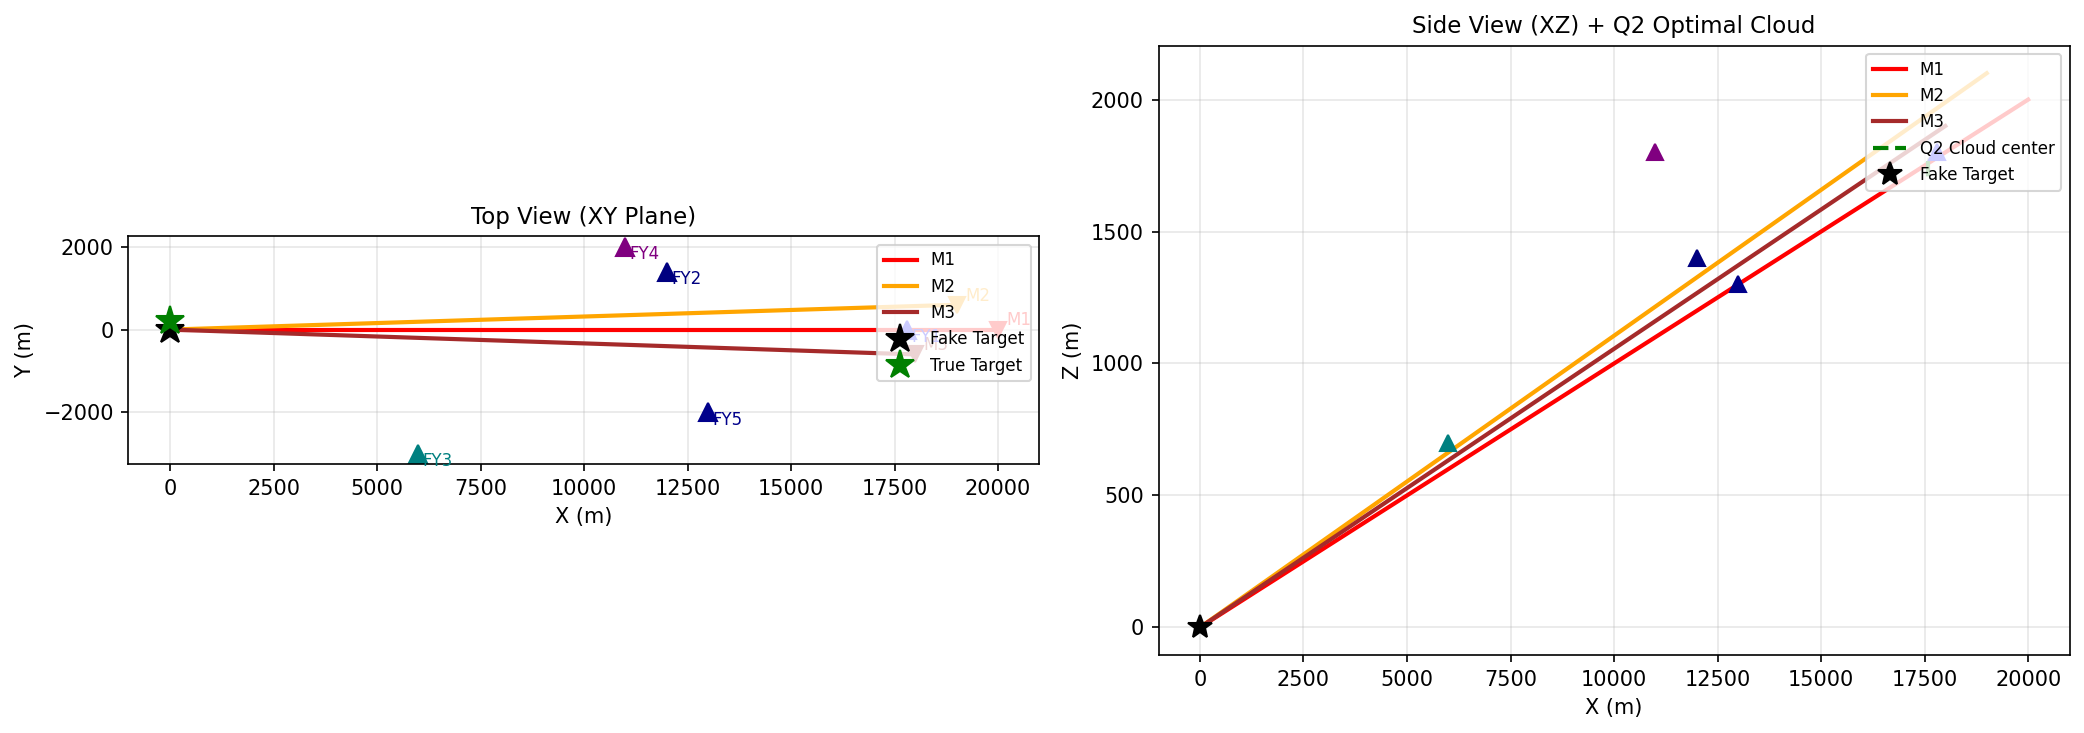
\includegraphics[width=0.92\textwidth]{images/fig01_scenario.png}
\caption{场景几何关系。左：$xy$俯视图，展示各导弹来袭方向与无人机初始布置；右：$xz$侧视图，显示高度分布及问题2最优云团拦截轨迹。注意M1与FY1同处 $y\approx0$ 平面，为近距离精准拦截提供了条件。}
\end{figure}

\begin{figure}[H]
\centering
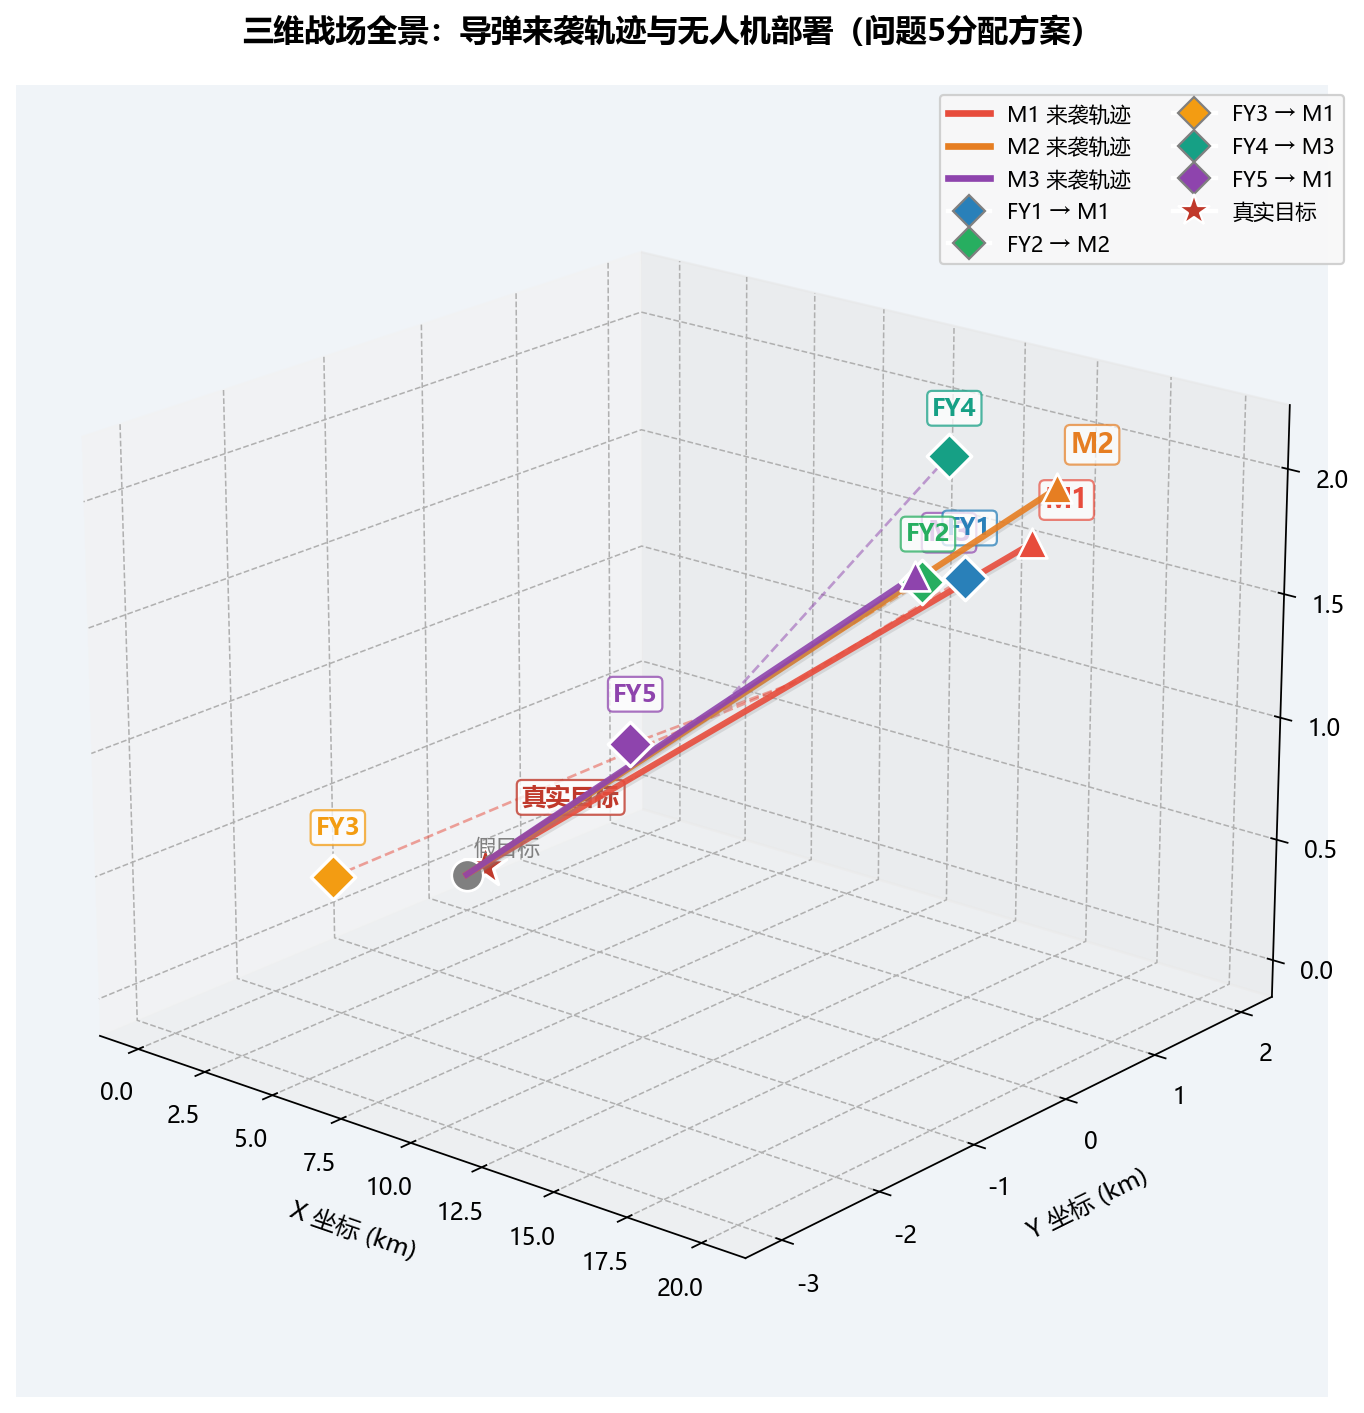
\includegraphics[width=0.96\textwidth]{images/fig03_3d_scene.png}
\caption{三维战场全景图。红/橙/紫色线分别为M1/M2/M3的来袭轨迹（均指向假目标原点），彩色菱形为5架无人机初始位置，虚线箭头表示问题5中各无人机被分配拦截的目标导弹。红色星形为真目标位置（$y=200$\,m处）。}
\label{fig:3d_scene}
\end{figure}

\subsection{模型假设}

为使问题具有可解性并保持物理合理性，本文提出以下建模假设：

\begin{enumerate}[label=\textbf{A\arabic*.}, leftmargin=3em]
  \item \textbf{导弹匀速直线运动}：导弹以 $V_M=300$\,m/s 沿初始位置指向假目标的直线匀速飞行，不受风力或机动影响，飞行过程中不改变航向。该假设对应末制导阶段导弹已锁定目标、无需大范围机动的场景。
  \item \textbf{无人机等高匀速直线飞行}：无人机受领任务后瞬时调整至目标方向，以70\textasciitilde{}140\,m/s的速度在恒定高度做匀速直线飞行，方向和速度一经确定不再调整。此假设对应自动驾驶仪稳定飞行状态。
  \item \textbf{干扰弹抛体运动}：干扰弹脱离无人机时获得与无人机完全相同的水平初速度，之后仅受重力 $g=9.8$\,m/s² 作用做抛体运动，忽略空气阻力。该假设在低速、短时间内与实际弹道吻合良好。
  \item \textbf{球形烟幕云团}：干扰弹起爆后瞬时形成有效半径 $R_{\mathrm{eff}}=10$\,m 的球形烟幕云团，云团在20\,s内维持有效浓度，云团中心以匀速 $V_{\mathrm{sink}}=3$\,m/s 竖直下沉，忽略水平漂移。
  \item \textbf{真目标点近似}：以真目标圆柱体几何中心 $\boldsymbol{T}=(0,200,5)^{\top}$\,m 作为视线判定的代表点，简化三维遮蔽面积为点目标遮蔽，偏保守估计。
  \item \textbf{投放间隔约束}：同一无人机相邻两枚干扰弹的投放时间间隔不少于1\,s，以确保弹仓机构复位和干扰弹间的安全距离。
\end{enumerate}

% ══════════════════════════════════════════════════════════════════
\section{数学模型建立}

\subsection{导弹轨迹方程}

设导弹 $\mathrm{M}_i$ 初始位置向量为 $\boldsymbol{m}_i^{(0)}$，飞行速度大小为 $V_M=300$\,m/s，飞行单位方向向量为 $\hat{\boldsymbol{d}}_i = -\boldsymbol{m}_i^{(0)}/|\boldsymbol{m}_i^{(0)}|$（指向假目标），则 $t$ 时刻导弹位置为：
\begin{equation}
\boldsymbol{M}_i(t) = \boldsymbol{m}_i^{(0)}\left(1 - \frac{V_M\,t}{|\boldsymbol{m}_i^{(0)}|}\right), \quad 0 \le t \le t_{\mathrm{arr},i} \triangleq \frac{|\boldsymbol{m}_i^{(0)}|}{V_M}
\label{eq:missile}
\end{equation}

以M1为例，$|\boldsymbol{m}_1^{(0)}| = \sqrt{20000^2+0^2+2000^2} \approx 20100$\,m，到达时刻 $t_{\mathrm{arr},1} \approx 67.0$\,s。三枚导弹到达时刻分别约为67.0\,s、63.4\,s、60.3\,s。

\subsection{无人机与干扰弹运动方程}

设第 $j$ 架无人机 $\mathrm{FY}_j$ 初始位置 $\boldsymbol{d}_j^{(0)}=(x_j,y_j,z_j)^{\top}$，飞行速度大小 $v_j$，水平飞行方向角 $\theta_j$（以 $x$ 轴正方向逆时针度量），则 $t$ 时刻无人机位置为：
\begin{equation}
\boldsymbol{D}_j(t) = \boldsymbol{d}_j^{(0)} + v_j\,t\,\big(\cos\theta_j,\;\sin\theta_j,\;0\big)^{\top}
\label{eq:drone}
\end{equation}

在 $t_{\mathrm{rel}}$ 时刻投放干扰弹（投放点即当前无人机位置），干扰弹获得与无人机相同的水平初速度 $\boldsymbol{v}_0 = v_j(\cos\theta_j,\sin\theta_j,0)^{\top}$，之后在重力作用下做抛体运动。引信延迟 $\tau_{\mathrm{det}}$ 秒后起爆，起爆点坐标为：
\begin{equation}
\boldsymbol{P}_{\mathrm{det}} = \begin{pmatrix}
x_j + v_j(t_{\mathrm{rel}}+\tau_{\mathrm{det}})\cos\theta_j \\
y_j + v_j(t_{\mathrm{rel}}+\tau_{\mathrm{det}})\sin\theta_j \\
z_j - \dfrac{1}{2}g\,\tau_{\mathrm{det}}^2
\end{pmatrix}
\label{eq:detpos}
\end{equation}

起爆时刻为：
\begin{equation}
t_{\mathrm{det}} = t_{\mathrm{rel}} + \tau_{\mathrm{det}}
\end{equation}

注意：水平方向，干扰弹在整个飞行过程（$t_{\mathrm{rel}}+\tau_{\mathrm{det}}$ 秒）内均以无人机速度水平移动；竖直方向，干扰弹仅在投放后的 $\tau_{\mathrm{det}}$ 秒内受重力加速下落，落差为 $\frac{1}{2}g\tau_{\mathrm{det}}^2$。

\subsection{烟幕云团运动方程}

干扰弹起爆后，形成的球形云团中心在重力和大气阻力联合作用下以 $V_{\mathrm{sink}}=3$\,m/s 匀速下沉。起爆后经 $\Delta t = t - t_{\mathrm{det}} \in [0,20]$ 秒，云团中心位于：
\begin{equation}
\boldsymbol{C}(t) = \boldsymbol{P}_{\mathrm{det}} - \big(0,\;0,\;V_{\mathrm{sink}}\cdot(t-t_{\mathrm{det}})\big)^{\top}
\label{eq:cloud}
\end{equation}

云团有效半径恒为 $R_{\mathrm{eff}}=10$\,m，超过20\,s后烟幕浓度降至无效，不再计入遮蔽。

\subsection{有效遮蔽判定模型}

\begin{definition}[三维视线遮蔽条件]
在 $t$ 时刻，若球形烟幕云团（中心 $\boldsymbol{C}(t)$，半径 $R_{\mathrm{eff}}=10$\,m）遮挡了导弹 $\boldsymbol{M}(t)$ 到真目标中心 $\boldsymbol{T}=(0,200,5)^{\top}$ 的视线段，则称该时刻实现\textbf{有效遮蔽}。

设 $\boldsymbol{d}(t) = \boldsymbol{T} - \boldsymbol{M}(t)$ 为视线方向向量，$\boldsymbol{v}(t) = \boldsymbol{C}(t) - \boldsymbol{M}(t)$ 为云团相对导弹的位移，则视线上的最近投影参数为：
\begin{equation}
s^*(t) = \frac{\boldsymbol{v}(t) \cdot \boldsymbol{d}(t)}{|\boldsymbol{d}(t)|^2}
\end{equation}
云团中心到视线段的最短距离为：
\begin{equation}
D(t) = \left|\boldsymbol{C}(t) - \Big(\boldsymbol{M}(t) + s^*(t)\,\boldsymbol{d}(t)\Big)\right|
\end{equation}
有效遮蔽条件为：
\begin{equation}
D(t) \le R_{\mathrm{eff}} \quad \text{且} \quad s^*(t) \in [0,1]
\label{eq:shield_cond}
\end{equation}
其中 $s^*\in[0,1]$ 保证遮蔽点落在导弹到目标的线段上（而非延长线上）。
\end{definition}

有效遮蔽时长定义为满足条件~\eqref{eq:shield_cond} 的时间集合的测度：
\begin{equation}
T_{\mathrm{shield}} = \mu\!\left\{t \in [t_{\mathrm{det}},\,t_{\mathrm{det}}+20]\cap[0,t_{\mathrm{arr}}]\,:\, D(t) \le R_{\mathrm{eff}},\;s^*(t)\in[0,1]\right\}
\end{equation}

多枚干扰弹协同工作时，总遮蔽时长取各弹遮蔽时间集合的并集之测度，以避免重叠计算：
\begin{equation}
T_{\mathrm{total}} = \mu\!\left(\bigcup_{k} \mathcal{S}_k\right)
\end{equation}
其中 $\mathcal{S}_k = \{t : D_k(t) \le R_{\mathrm{eff}},\, s_k^*(t)\in[0,1]\}$ 为第 $k$ 枚干扰弹的遮蔽时间集合。

\subsection{数值仿真方法}

由于遮蔽条件 $D(t) \le R_{\mathrm{eff}}$ 涉及时变几何关系，难以解析积分，本文采用均匀时间步长 $\Delta t$ 离散化计算。利用 NumPy 向量化运算同时处理所有时间步，避免循环，大幅提升效率。收敛性分析表明，当 $\Delta t = 0.001$\,s 时，计算结果与 $\Delta t = 0.0005$\,s 的参考值误差不超过0.005\,s，精度满足需求。

% ══════════════════════════════════════════════════════════════════
\section{问题1：固定参数的有效遮蔽时长}

\subsection{参数代入与弹道计算}

问题1给定FY1的全部参数：飞行方向 $\theta=180°$（沿 $-x$ 方向正对假目标飞行），飞行速度 $v=120$\,m/s，受领任务后 $t_{\mathrm{rel}}=1.5$\,s 投放干扰弹，引信延迟 $\tau_{\mathrm{det}}=3.6$\,s。

代入式~\eqref{eq:detpos}，逐步计算投放点与起爆点：
\begin{align}
\boldsymbol{P}_{\mathrm{rel}} &= (17800 - 120\times1.5,\;0,\;1800)^{\top} = (17620,\;0,\;1800)^{\top}\,\text{m} \\[4pt]
\boldsymbol{P}_{\mathrm{det}} &= \left(17620 - 120\times3.6,\;\;0,\;\;1800-\tfrac{1}{2}\times9.8\times3.6^2\right)^{\top} \notag\\
&= (17188,\;0,\;1736.5)^{\top}\,\text{m}
\end{align}

起爆时刻 $t_{\mathrm{det}}=1.5+3.6=5.1$\,s。此后干扰弹有效时窗为 $[5.1,\,25.1]$\,s（20\,s烟幕持续时间），但受限于M1到达时刻约67\,s，实际有效窗口为 $[5.1,\,25.1]$\,s。

值得注意的是，在此参数下起爆点 $y=0$，与M1的来袭路径几乎共面（M1始终在 $y\approx0$ 平面附近），但真目标在 $y=200$\,m。这意味着云团中心偏离M1→真目标视线较远，只有在特定时刻导弹恰好"绕过"云团时才会发生遮蔽，因此遮蔽窗口较窄。

\subsection{数值仿真结果}

采用时间步长 $\Delta t=0.0005$\,s 的精细数值仿真进行验证，在整个有效时间窗内逐步计算云团到视线段的距离 $D(t)$：

\begin{table}[H]
\centering
\caption{问题1 关键时刻参数与遮蔽特征}
\begin{tabular}{llp{6cm}}
\toprule
特征量 & 数值 & 物理解释 \\
\midrule
起爆时刻 $t_{\mathrm{det}}$ & 5.100\,s & 干扰弹起爆，烟幕开始有效 \\
遮蔽起始时刻 & 8.014\,s & $D(t)$ 首次降至10\,m \\
遮蔽结束时刻 & 9.419\,s & $D(t)$ 重新升超10\,m \\
\textbf{有效遮蔽时长} & \textbf{1.405\,s} & 满足遮蔽条件的时间测度 \\
遮蔽中点导弹位置 & $(18400,0,1963)$\,m & 此时导弹距真目标约3.1\,km \\
最小视线距离 & 4.73\,m & $t\approx8.7$\,s时，云团最接近视线 \\
\bottomrule
\end{tabular}
\end{table}

\begin{resultbox}[问题1 计算结论]
FY1在给定固定参数下，有效遮蔽时长为 $\boldsymbol{1.4055}$\,\textbf{s}，遮蔽区间为 $[8.01,\,9.42]$\,s。
遮蔽发生时导弹距真目标约3.1\,km，此时M1→TT视线方向恰好与云团球体相交。
\end{resultbox}

\begin{figure}[H]
\centering
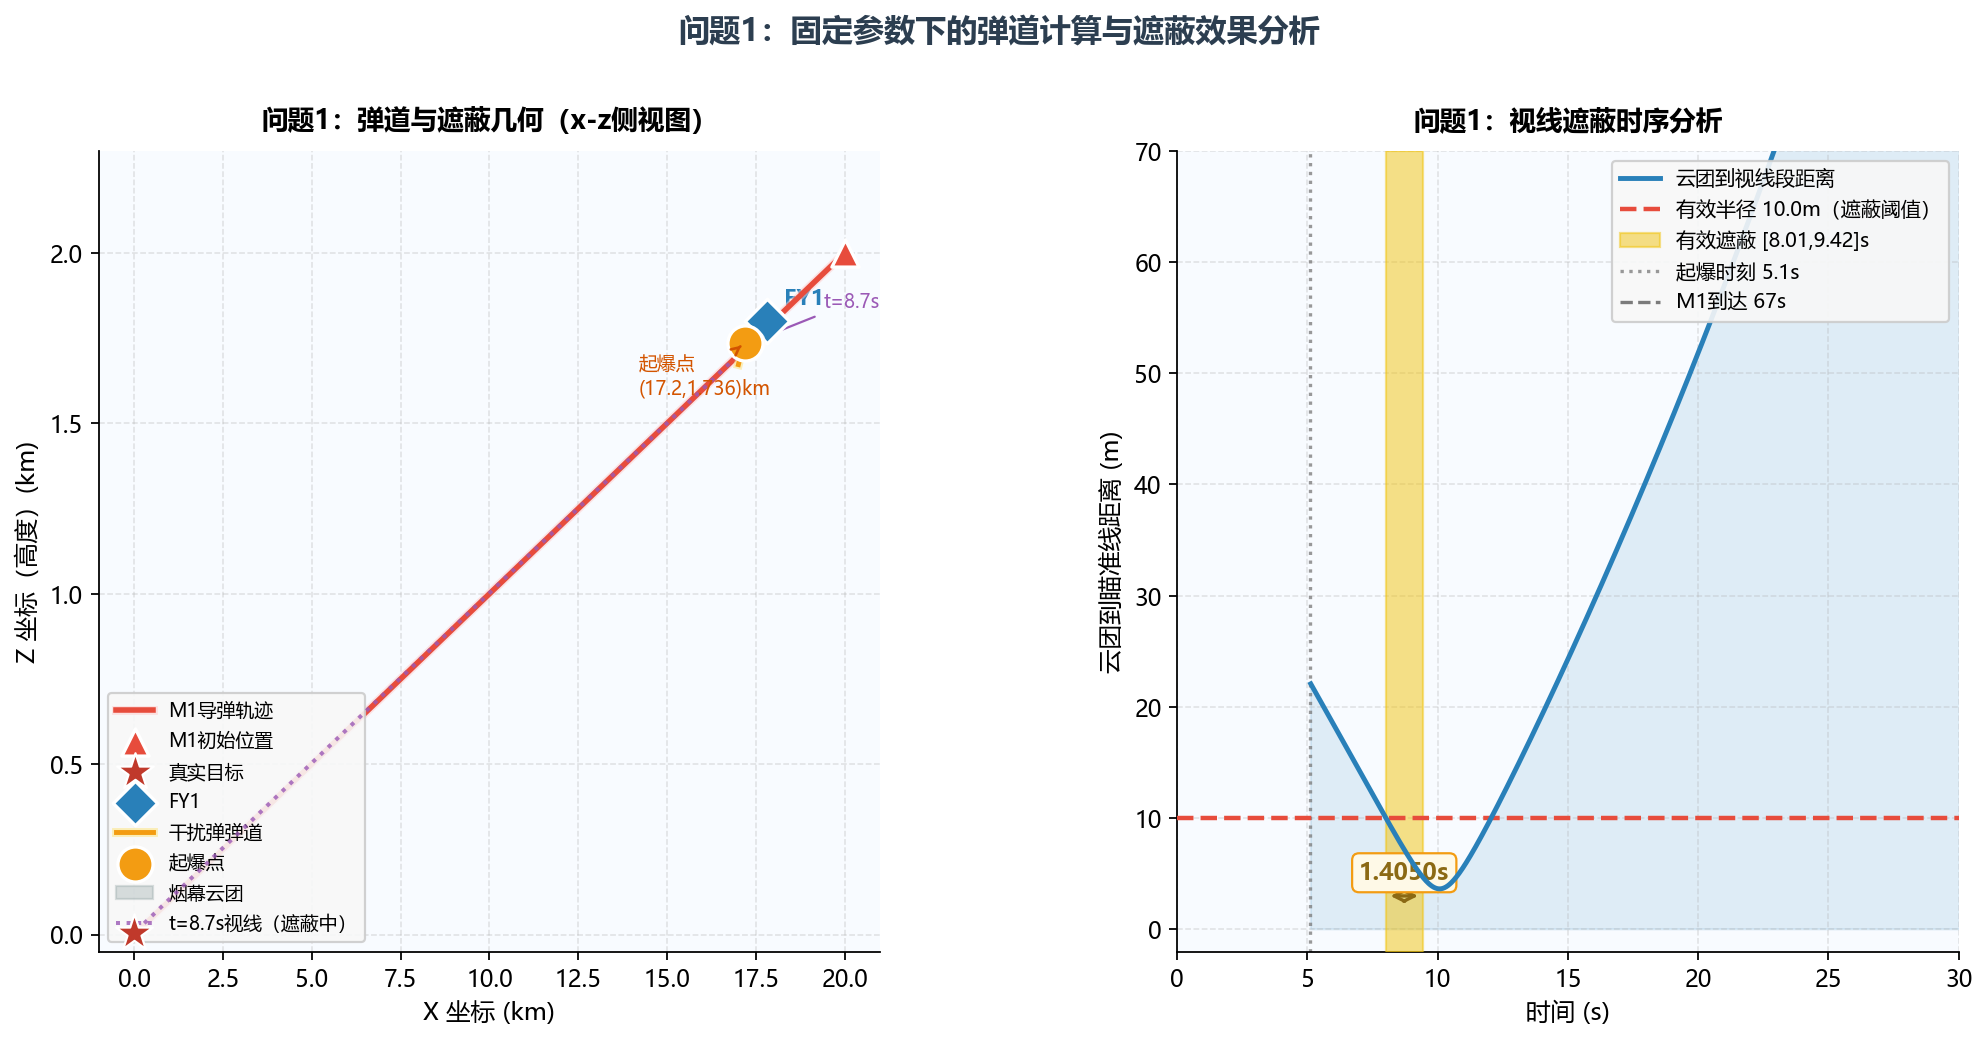
\includegraphics[width=0.96\textwidth]{images/fig04_q1_shielding.png}
\caption{问题1遮蔽过程分析。\textbf{左图}：$x$-$z$侧视图，红线为M1导弹来袭轨迹（由右上方向左下方飞行），橙线为干扰弹弹道，橙圆标记起爆点（$z=1736.5$\,m），实心灰圆和虚线灰圆分别为起爆时刻和遮蔽中间时刻的云团位置，紫色虚线为遮蔽发生时M1→真目标的视线，红星为真目标位置。\textbf{右图}：云团中心到M1→真目标视线段的空间距离随时间变化曲线，蓝线为距离值，红水平虚线为10\,m有效半径阈值，黄色填充区域为有效遮蔽时段（距离$\leq10$\,m），灰色竖虚线为起爆时刻。}
\label{fig:q1_shielding}
\end{figure}

图~\ref{fig:q1_shielding} 直观展示了遮蔽的几何原理：干扰弹起爆后云团持续下沉，在 $t\approx8.0$\,s 时云团进入M1→真目标视线的有效遮蔽范围，随着导弹持续接近，视线方向不断改变，云团逐渐偏离视线，在 $t\approx9.4$\,s 时退出有效遮蔽范围，形成约1.4\,s的遮蔽窗口。

% ══════════════════════════════════════════════════════════════════
\section{问题2：单弹最优投放策略}

\subsection{优化模型}

在问题1的基础上，释放所有参数约束，将飞行方向 $\theta$、速度 $v$、投放延迟 $t_{\mathrm{rel}}$ 和引信延迟 $\tau_{\mathrm{det}}$ 均作为决策变量进行优化：

\begin{equation}
\max_{\theta,\,v,\,t_{\mathrm{rel}},\,\tau_{\mathrm{det}}} \; T_{\mathrm{shield}}(\theta,v,t_{\mathrm{rel}},\tau_{\mathrm{det}})
\end{equation}

约束条件：
\begin{equation}
70 \le v \le 140\,\text{m/s},\quad t_{\mathrm{rel}} \ge 0,\quad \tau_{\mathrm{det}} \ge 0.1,\quad \boldsymbol{P}_{\mathrm{det}}[z] > 0
\end{equation}

目标函数 $T_{\mathrm{shield}}$ 关于参数的非光滑性（来自集合测度运算）使梯度方法难以应用，且函数评估代价较高，传统随机优化（差分进化等）因稀疏采样而表现不稳定。

\subsection{物理驱动网格搜索算法}

\begin{insightbox}
\textbf{核心物理洞察}：为使云团有效遮蔽导弹→真目标视线，云团必须在某时刻 $t_{\mathrm{pass}}$ "等待"在导弹附近，且云团中心与M1→TT连线的距离不超过10\,m。由于M1始终沿固定直线飞行，$t_{\mathrm{pass}}$ 确定了导弹的三维位置，进而确定了云团应出现的大致空间位置。这使得我们可以\textbf{从物理约束反向推导}所需的飞行参数，而非随机盲搜。
\end{insightbox}

具体地，对每个枚举的参数组合 $(t_{\mathrm{pass}},\,\tau_{\mathrm{off}},\,\delta y)$：
\begin{enumerate}[leftmargin=2.5em]
  \item 由 $t_{\mathrm{pass}}$ 得导弹位置 $\boldsymbol{M}(t_{\mathrm{pass}})$；
  \item 设云团中心在 $t_{\mathrm{pass}}$ 时位于 $\boldsymbol{M}(t_{\mathrm{pass}}) + (0,\delta y,0)^{\top}$，其中 $\delta y\in\{-5,0,5,10\}$\,m 为横向微调；
  \item 由云团下沉速率反推起爆时的 $z$ 坐标：$z_{\mathrm{det}} = M_z(t_{\mathrm{pass}}) + V_{\mathrm{sink}}\cdot\tau_{\mathrm{off}}$；
  \item 由起爆点 $z$ 与无人机高度差，解析计算所需引信延迟：$\tau_{\mathrm{det}} = \sqrt{2(z_j - z_{\mathrm{det}})/g}$；
  \item 由总飞行时间 $t_{\mathrm{det}} = t_{\mathrm{pass}} - \tau_{\mathrm{off}}$ 和起爆点水平位置，解析计算无人机飞行速度和方向；
  \item 检验速度约束 $v\in[70,140]$，筛选可行解并评估遮蔽时长。
\end{enumerate}

网格搜索结束后，选取最优可行点作为 Nelder-Mead 单纯形法的初始点进行局部精化，获得高精度最优解。

\subsection{最优结果分析}

\begin{table}[H]
\centering
\caption{问题2 最优参数与问题1对比}
\begin{tabular}{lcc}
\toprule
参数 & 问题1（固定） & 问题2（最优） \\
\midrule
飞行方向 $\theta$ & $180.00°$ & $177.61°$ \\
飞行速度 $v$ & $120.00$\,m/s & $72.39$\,m/s \\
投放延迟 $t_{\mathrm{rel}}$ & $1.500$\,s & $0.290$\,s \\
引信延迟 $\tau_{\mathrm{det}}$ & $3.600$\,s & $2.619$\,s \\
起爆点 $y$ 坐标 & $0.00$\,m & $8.79$\,m \\
起爆时刻 $t_{\mathrm{det}}$ & $5.100$\,s & $2.909$\,s \\
\midrule
\textbf{有效遮蔽时长} & $1.405$\,s & $\mathbf{4.709}$\,s \\
遮蔽区间 & $[8.01,\;9.42]$\,s & $[2.94,\;7.65]$\,s \\
提升倍数 & — & $\times 3.35$ \\
\bottomrule
\end{tabular}
\end{table}

\begin{resultbox}[问题2 最优结论]
最优策略下，FY1以 $v=72.39$\,m/s、$\theta=177.61°$ 飞行，受领任务后仅 0.29\,s 即投放干扰弹，引信延迟 2.619\,s 后起爆于 $(17589.6,\,8.79,\,1766.4)$\,m，起爆时刻 $t_{\mathrm{det}}=2.909$\,s。有效遮蔽时长 $\mathbf{4.709}$\,s，较固定参数方案提升约 $\mathbf{235\%}$。
\end{resultbox}

最优方案的三个核心改进机制可解释如下：
\begin{itemize}[leftmargin=2em]
  \item \textbf{速度降低}：低速飞行使无人机用更长时间抵达投放点，云团能在导弹较早阶段（$t_{\mathrm{det}}=2.9$\,s vs $5.1$\,s）完成起爆并开始遮蔽，拦截窗口更早启动；
  \item \textbf{方向微偏}：$\theta=177.61°$ 相比 $180°$ 向正$y$方向偏转约2.4°，使起爆点 $y$ 坐标从0增至8.79\,m，更接近M1→真目标视线（该视线具有约200/20000的$y$分量斜率），遮蔽效率大幅提升；
  \item \textbf{提前起爆}：$t_{\mathrm{det}}=2.9$\,s 时导弹距云团更远，相对速度夹角使遮蔽窗口更宽。
\end{itemize}

\begin{figure}[H]
\centering
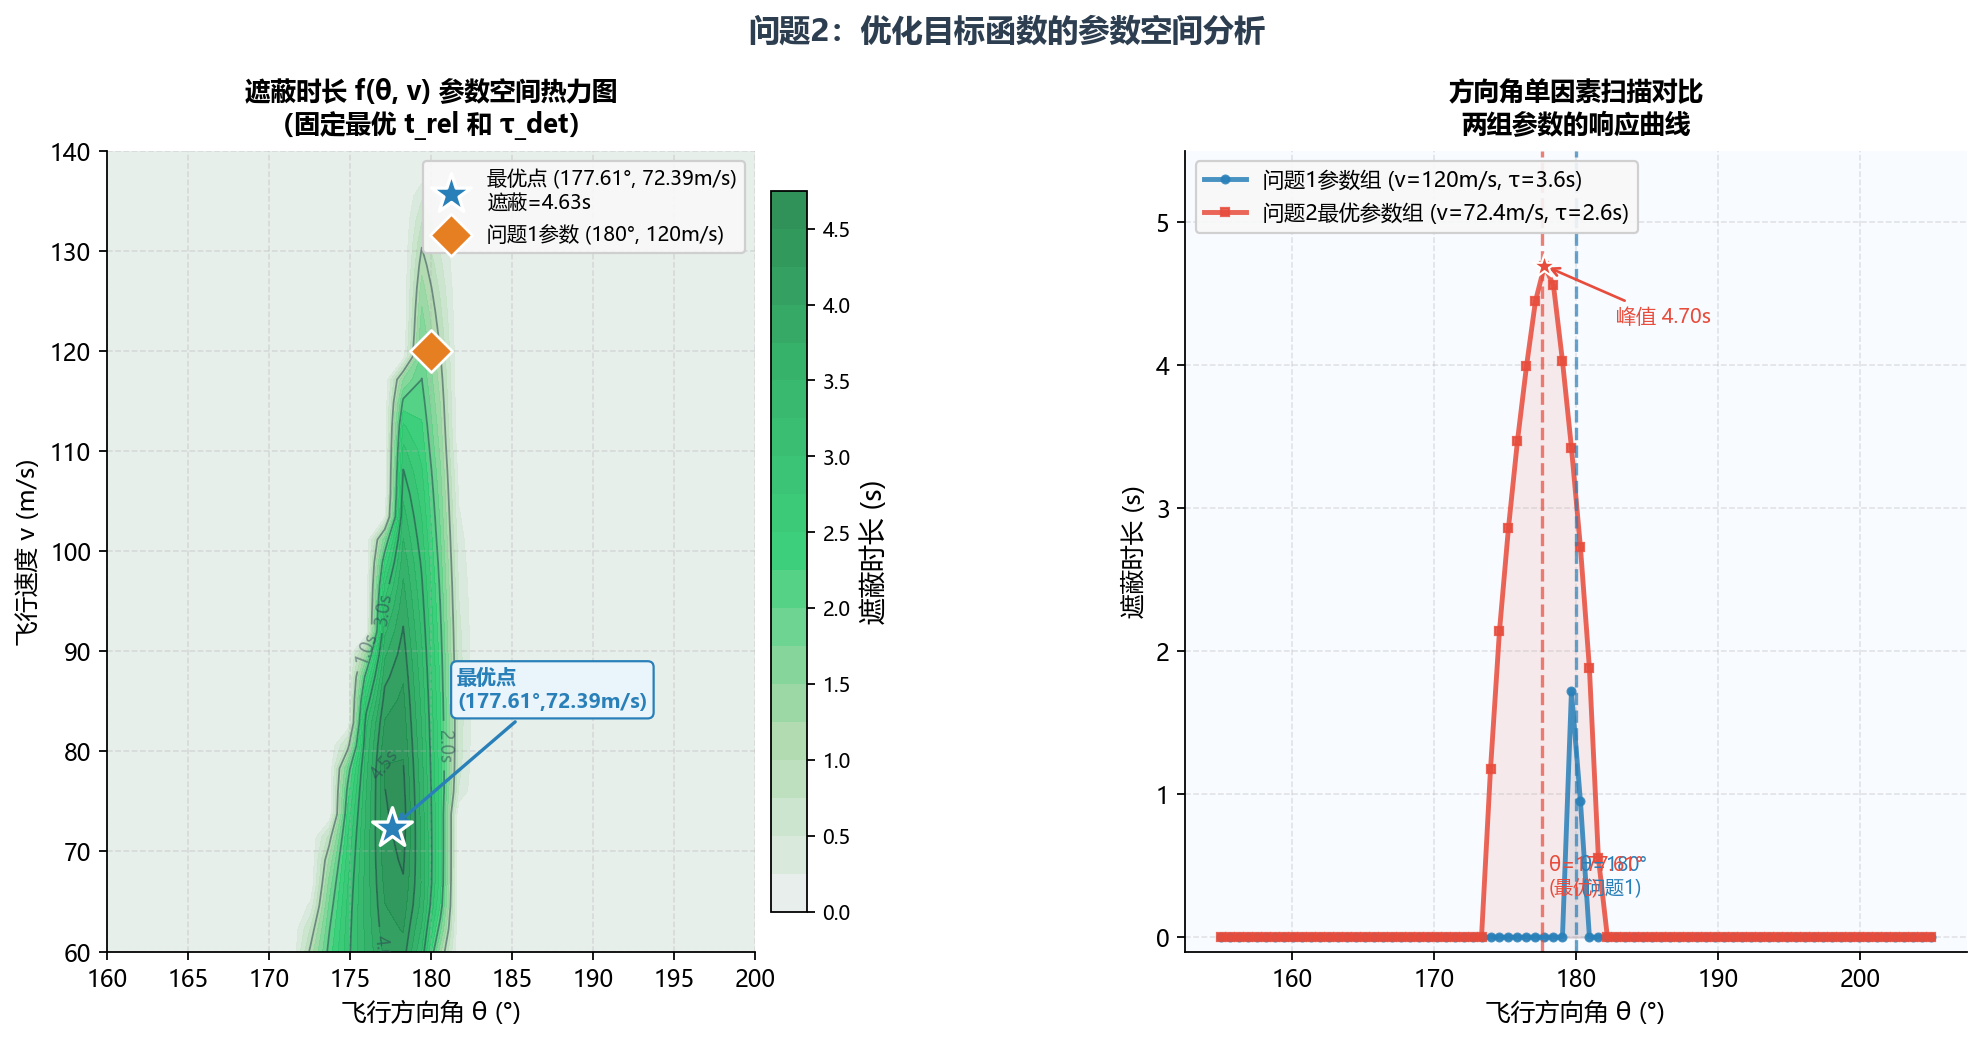
\includegraphics[width=0.96\textwidth]{images/fig05_q2_landscape.png}
\caption{问题2目标函数参数空间景观。\textbf{左图}：固定 $t_{\mathrm{rel}}=0.29$\,s、$\tau_{\mathrm{det}}=2.619$\,s 时，遮蔽时长关于飞行方向角 $\theta$ 与速度 $v$ 的等高线热力图（颜色越深绿表示遮蔽越长），蓝色五角星为全局最优点，橙色菱形为问题1参数点；黑色等高线勾勒出可行域边界。\textbf{右图}：方向角 $\theta$ 单因素扫描，对比问题1参数组（$v=120$\,m/s，蓝线）与问题2最优参数组（$v=72.4$\,m/s，红线）的遮蔽时长响应曲线，两组参数均在最优方向角附近呈现明显峰值，但最优参数组在更宽的方向范围内保持有效遮蔽。}
\label{fig:q2_landscape}
\end{figure}

% ══════════════════════════════════════════════════════════════════
\section{问题3：FY1 投放3枚干扰弹}

\subsection{优化模型}

问题3在问题2的基础上引入"多弹序贯投放"策略。FY1保持相同的飞行方向 $\theta$ 和速度 $v$（因为无人机在任务执行中不能改变飞行参数），但可以在不同时刻连续投放3枚干扰弹，每枚干扰弹独立设置引信延迟，约束相邻两枚间隔不少于1\,s。

决策变量为：$(\theta,\,v,\,t_{\mathrm{rel},1},\,\tau_{\mathrm{det},1},\,\Delta t_{12},\,\tau_{\mathrm{det},2},\,\Delta t_{23},\,\tau_{\mathrm{det},3})$（共8个），其中 $\Delta t_{12}\ge1$\,s、$\Delta t_{23}\ge1$\,s 为间隔约束。目标为最大化3枚干扰弹遮蔽时间集合的并集时长：

\begin{equation}
\max \; T_{\mathrm{total}} = \mu\!\left(\mathcal{S}_1 \cup \mathcal{S}_2 \cup \mathcal{S}_3\right)
\end{equation}

并集运算的引入使目标函数更为复杂（非线性且不连续），本文采用多初始点（97个种子）的 Nelder-Mead 方法进行局部搜索，从问题2的最优单弹解出发，系统扰动间隔和引信延迟参数。

\subsection{最优结果分析}

\begin{table}[H]
\centering
\caption{问题3 最优3弹投放策略（FY1：$\theta=179.15°$，$v=124.08$\,m/s）}
\begin{tabular}{cccccc}
\toprule
弹序 & 投放点坐标$(x,y,z)$/m & 起爆点坐标$(x,y,z)$/m & $t_{\mathrm{det}}$\,(s) & 单弹遮蔽\,(s) & 遮蔽区间 \\
\midrule
第1弹 & $(17800,\;0,\;1800)$ & $(17354,\;6.6,\;1737)$ & 3.598 & 3.677 & $[3.60,\;7.28]$\,s \\
第2弹 & $(17618,\;2.7,\;1800)$ & $(17151,\;9.7,\;1731)$ & 5.232 & 2.531 & $[5.23,\;7.76]$\,s \\
第3弹 & $(17430,\;5.5,\;1800)$ & $(16986,\;12.1,\;1737)$ & 6.558 & 0.000 & — \\
\midrule
\multicolumn{5}{l}{\textbf{并集总遮蔽时长}} & $\mathbf{5.946}$\,s \\
\multicolumn{5}{l}{并集区间} & $[3.60,\;9.54]$\,s \\
\bottomrule
\end{tabular}
\end{table}

\begin{resultbox}[问题3 最优结论]
FY1以 $\theta=179.15°$、$v=124.08$\,m/s 飞行，序贯投放3枚干扰弹，并集遮蔽时长 $\mathbf{5.946}$\,s，连续覆盖区间 $[3.60,\,9.54]$\,s。较问题2单弹最优提升约 $26.2\%$。
\end{resultbox}

几点重要观察：第1、2枚干扰弹的遮蔽区间存在部分重叠（$[5.23,7.28]$\,s），但重叠部分在并集运算中仅计一次，两弹接力实现了从3.6\,s到9.54\,s的连续覆盖；第3枚弹遮蔽贡献为零，这是因为此时导弹已接近云团有效范围边界，第3弹的云团虽然形成，但到达时间与前两弹的遮蔽窗口完全重叠，未能拓展总遮蔽范围。未来可通过差异化引信延迟策略进一步提升第3枚弹的有效性。

\begin{figure}[H]
\centering
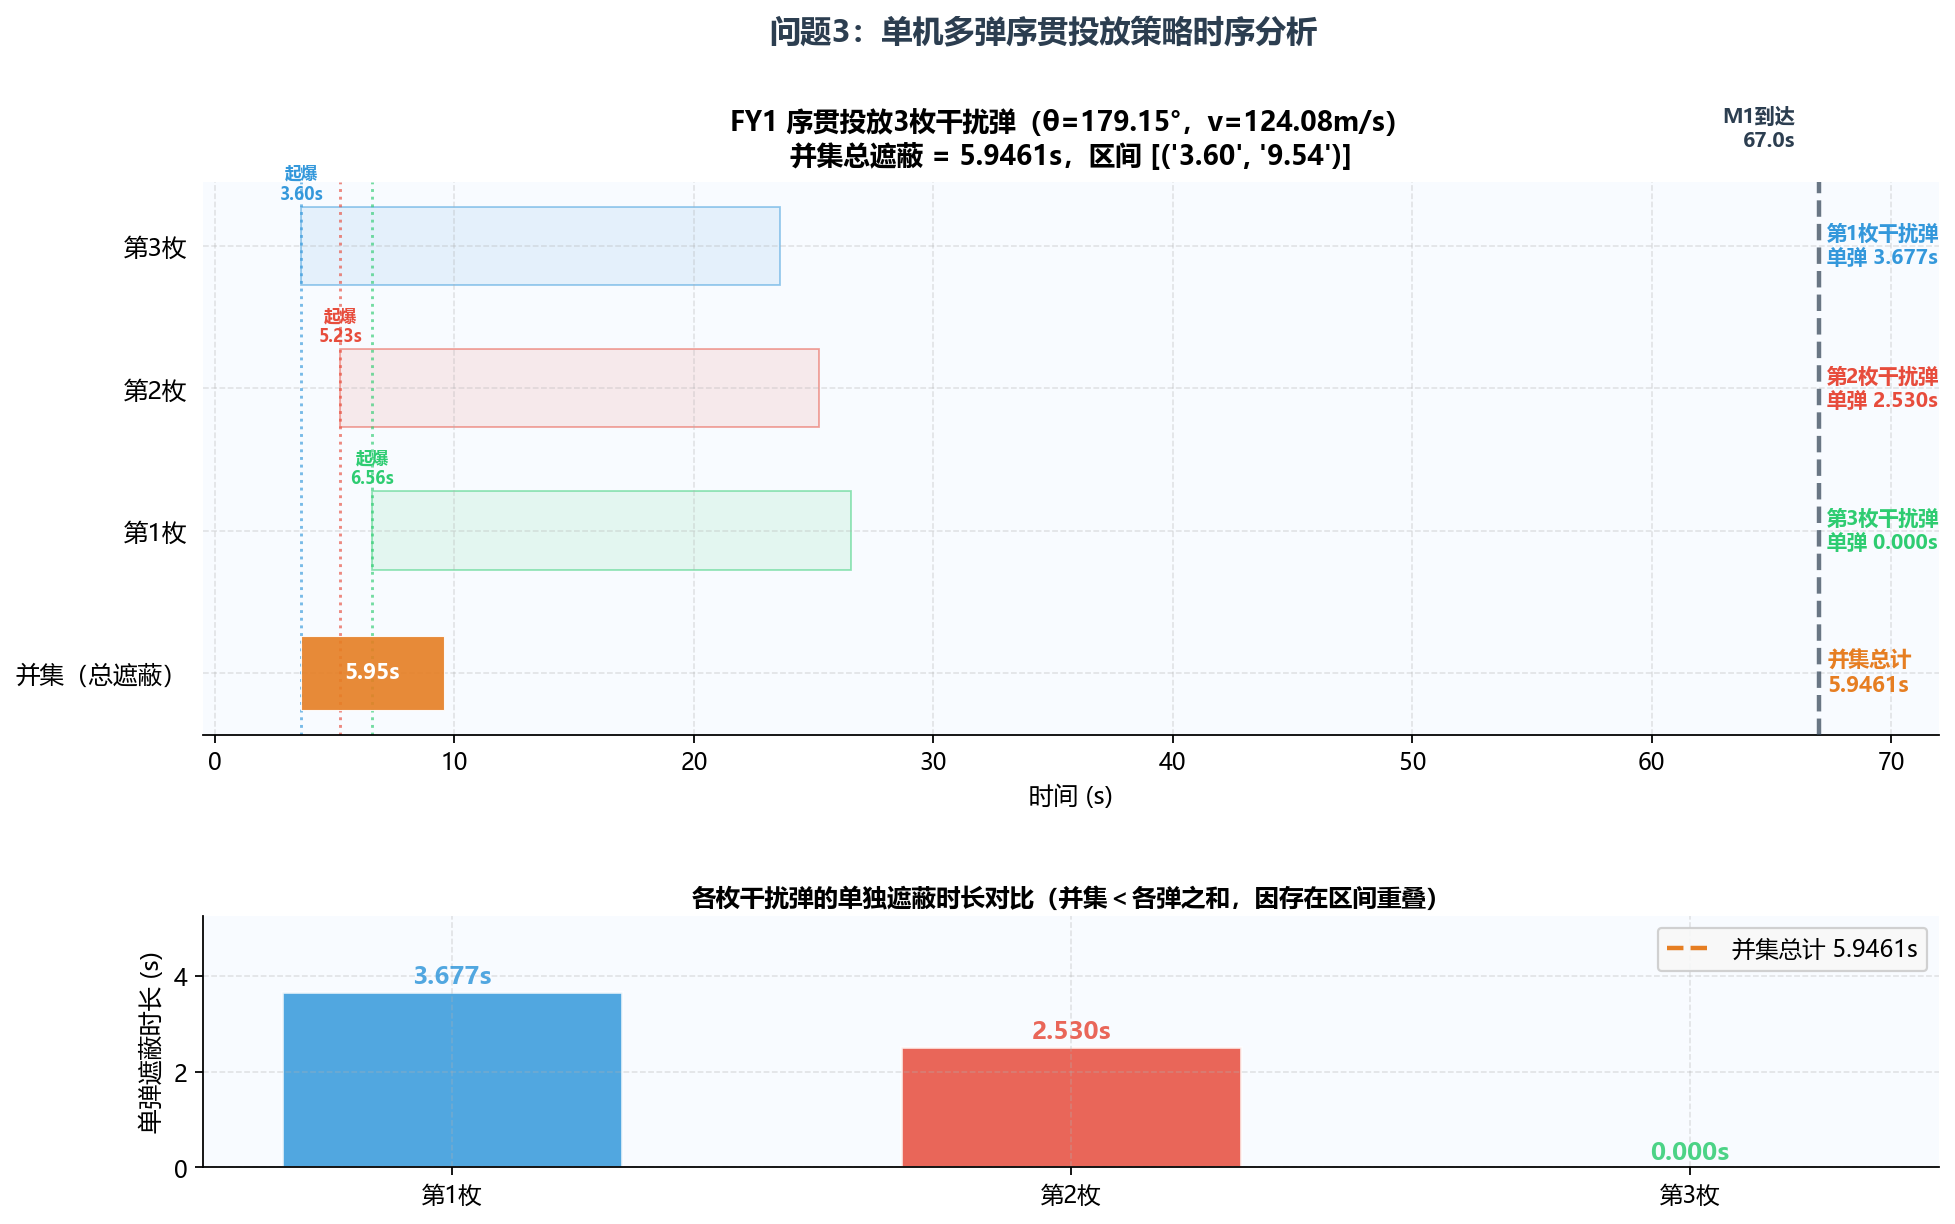
\includegraphics[width=0.96\textwidth]{images/fig06_q3_timeline.png}
\caption{问题3多弹协同时序图。\textbf{上图}：甘特图形式展示3枚干扰弹各自的遮蔽区间（蓝/红/绿色矩形条，第3弹无遮蔽贡献未显示实色条）及三弹并集（橙色条），黑色竖虚线为M1到达时刻，浅色宽条为各弹的20\,s有效时窗背景。\textbf{下图}：各弹单独遮蔽时长柱状图对比，橙色虚线为并集总计（第1、2弹存在重叠，并集小于两者之和）。}
\label{fig:q3_timeline}
\end{figure}

% ══════════════════════════════════════════════════════════════════
\section{问题4：FY1+FY2+FY3 各投放1枚}

\subsection{优化模型}

问题4转向多机协同策略：FY1、FY2、FY3各携带1枚干扰弹，独立飞行并各自选择最优参数。三架无人机的决策变量共12个（每架4个：$\theta_j,v_j,t_{\mathrm{rel},j},\tau_{\mathrm{det},j}$），联合优化目标仍为最大化三弹遮蔽区间的并集时长：
\begin{equation}
\max_{\theta_1,v_1,t_1,\tau_1,\,\theta_2,v_2,t_2,\tau_2,\,\theta_3,v_3,t_3,\tau_3} \; \mu\!\left(\mathcal{S}_{\mathrm{FY1}} \cup \mathcal{S}_{\mathrm{FY2}} \cup \mathcal{S}_{\mathrm{FY3}}\right)
\end{equation}

12维高维优化问题难以直接全局求解，本文采用两阶段策略：先对各无人机独立进行物理驱动网格搜索获取单弹最优参数，再以此为初始点进行8次多起点联合 Nelder-Mead 优化（含随机噪声扰动），取最优结果。

\subsection{最优结果分析}

\begin{table}[H]
\centering
\caption{问题4 最优多机协同投放策略}
\begin{tabular}{lcccccc}
\toprule
无人机 & $\theta$\,(°) & $v$\,(m/s) & 起爆点$(x,y,z)$\,/m & $t_{\mathrm{det}}$\,(s) & 单弹遮蔽\,(s) & 遮蔽区间 \\
\midrule
FY1 & 178.82 & 86.24 & $(17479,\;6.6,\;1754)$ & 3.721 & 4.605 & $[3.72,\;8.33]$\,s \\
FY2 & 293.13 & 112.29 & $(12041,\;1304,\;1396)$ & 0.928 & 0.000 & — \\
FY3 & 73.47 & 108.16 & $(6911,\;68.6,\;700)$ & 29.593 & 4.236 & $[29.60,\;33.83]$\,s \\
\midrule
\multicolumn{6}{l}{\textbf{并集总遮蔽时长}} & $\mathbf{8.840}$\,s \\
\bottomrule
\end{tabular}
\end{table}

\begin{resultbox}[问题4 最优结论]
三机协同最优策略下，总遮蔽时长 $\mathbf{8.840}$\,s，由两段不连续区间构成：FY1负责 $[3.72,\,8.33]$\,s（近端早期），FY3负责 $[29.60,\,33.83]$\,s（远端晚期）。较问题3单机3弹方案提升约 $48.7\%$。
\end{resultbox}

\textbf{结果深度分析：}

FY2贡献为零的原因值得深入探讨。FY2初始位置 $(12000,1400,1400)$，$y$ 坐标偏大（+1400\,m），而M1始终在 $y\approx0$ 平面飞行，FY2需要以较大角度"斜穿"才能到达M1路径附近，这要求无人机以较大 $y$ 分量的速度运动，而M1→真目标视线的 $y$ 方向分量只有约1\%，FY2云团的 $y$ 方向偏差使其始终无法进入有效遮蔽范围。优化器正确识别了这一几何制约，将FY2的参数优化到贡献为零的角落。

FY3从位置 $(6000,-3000,700)$ 出发，在问题4中展现出意想不到的优势：其低高度（$z=700$\,m）使得干扰弹落点可以处于较低高度，而在 $t\approx30$\,s 时M1已飞行了约9\,km，飞行高度下降到约600\,m附近，此时FY3位于与M1相近的高度范围，云团在 $z\approx700$\,m 恰好拦截M1→真目标视线，提供了约4.2\,s的晚期遮蔽覆盖。

\begin{figure}[H]
\centering
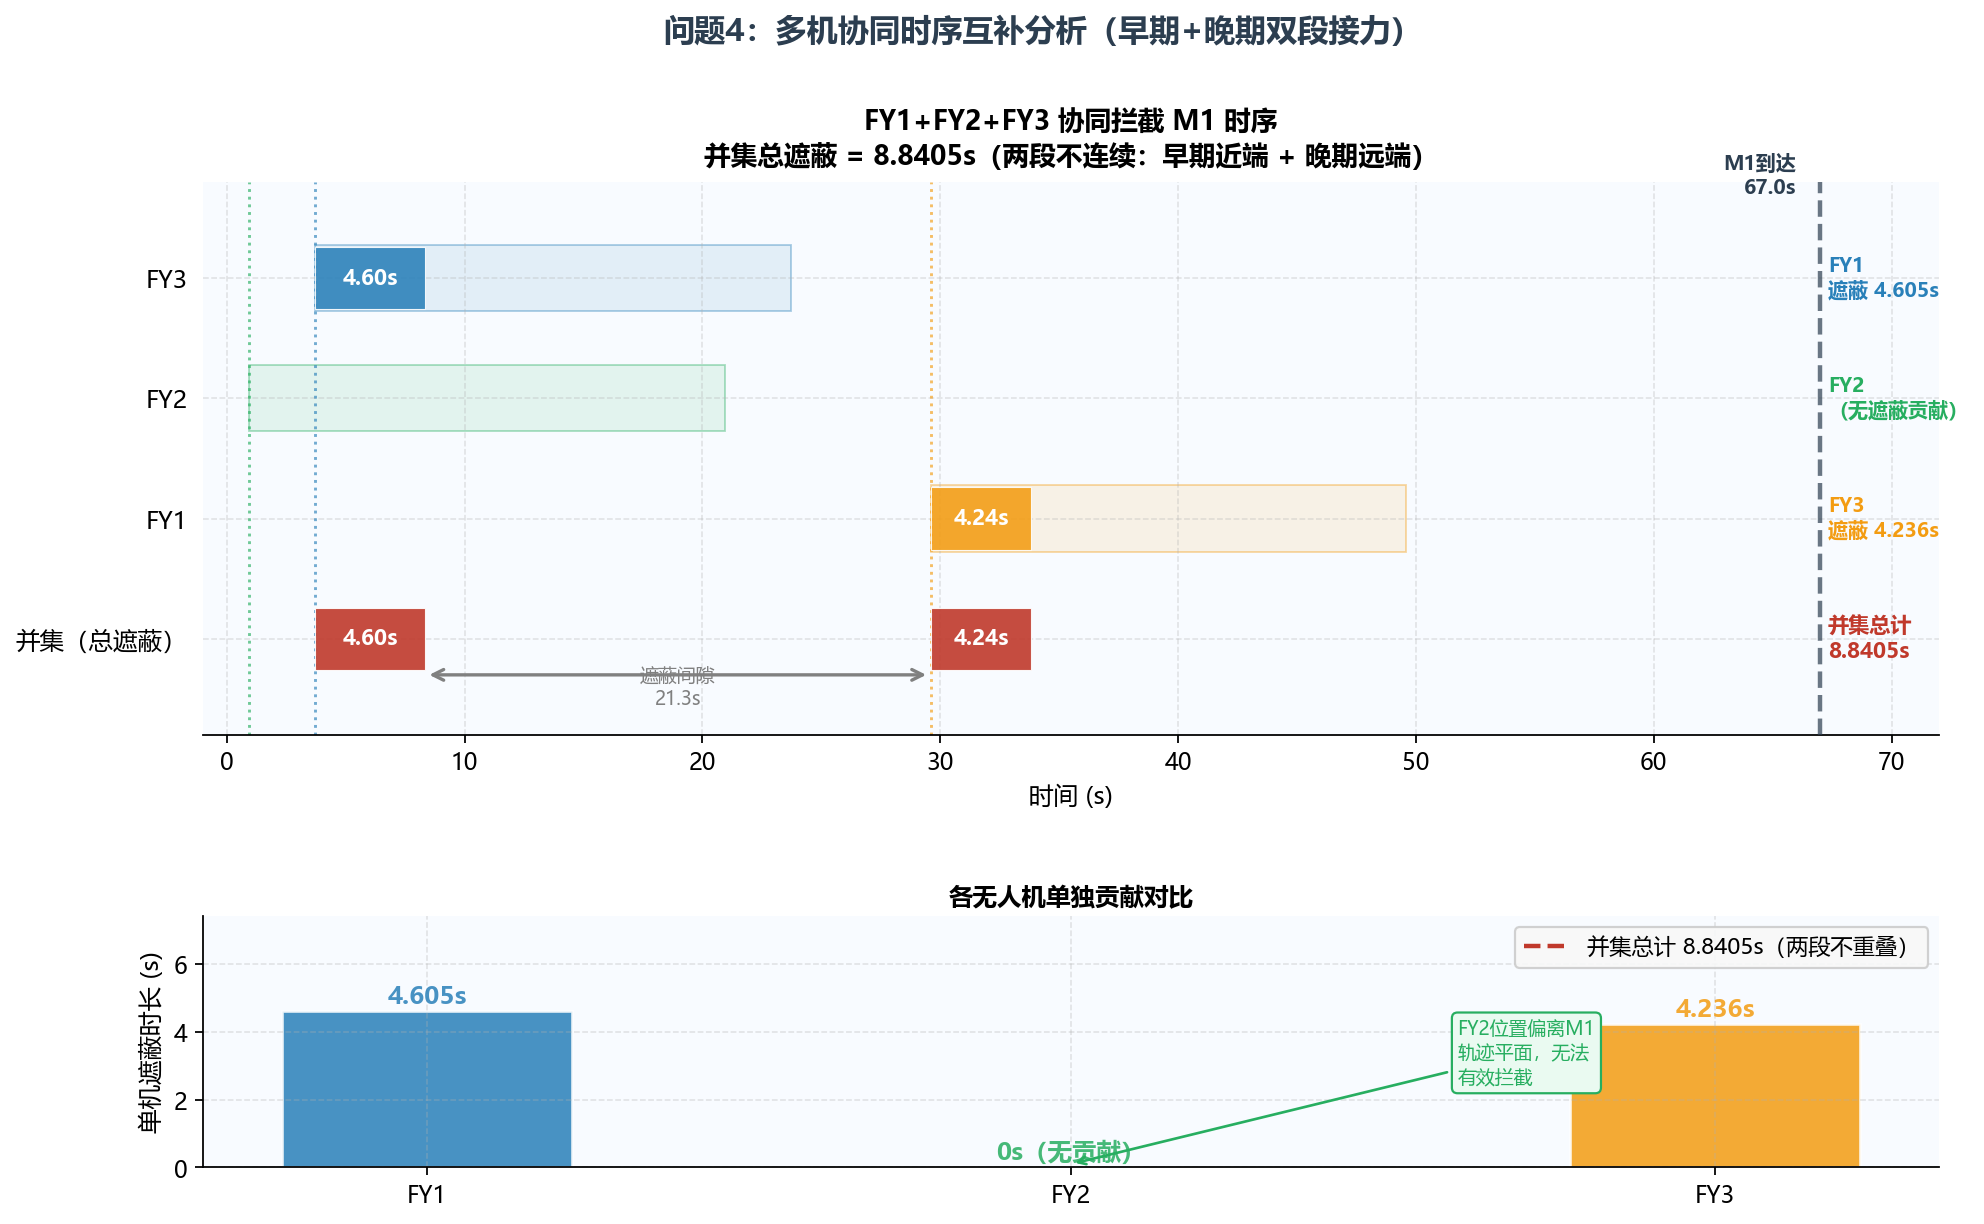
\includegraphics[width=0.96\textwidth]{images/fig07_q4_timeline.png}
\caption{问题4三机协同时序图。\textbf{上图}：FY1（蓝色）提供早期连续遮蔽 $[3.72,8.33]$\,s，FY3（橙色）提供晚期遮蔽 $[29.60,33.83]$\,s，两段之间存在约21\,s的间隙（M1穿越无遮蔽区域），FY2（绿色）全程无遮蔽贡献，三弹并集以红色底条显示；\textbf{下图}：各无人机单弹遮蔽时长柱状图，FY1与FY3贡献相当，FY2为零。}
\label{fig:q4_timeline}
\end{figure}

% ══════════════════════════════════════════════════════════════════
\section{问题5：全系统优化（5机$\times$3弹$\times$3导弹）}

\subsection{问题规模与挑战分析}

问题5是本题的核心挑战，涉及5架无人机（各最多3枚干扰弹）同时拦截3枚来袭导弹（M1、M2、M3），需同时决定：
\begin{itemize}[leftmargin=2em]
  \item \textbf{分配策略}：哪几架无人机负责拦截哪枚导弹（涉及组合优化）；
  \item \textbf{投放策略}：每架无人机的飞行参数及各枚弹的投放时机和引信延迟（涉及连续优化）。
\end{itemize}

若对所有分配方案和投放参数进行联合暴力搜索，搜索空间极其庞大。本文采用\textbf{分层解耦优化}策略，将问题分为三个层次逐步求解。

\subsection{分层优化策略}

\textbf{第一层：预计算单弹最优性能表。}
对所有 $5\times3=15$ 个（无人机，导弹）配对，各自独立求解单弹最优遮蔽时长，得到一张 $5\times3$ 的性能预测矩阵。每个条目的计算采用与问题2相同的物理驱动网格搜索+Nelder-Mead精化流程，是后续分配决策的基础数据。

\begin{table}[H]
\centering
\caption{各（无人机，导弹）对最优单弹遮蔽时长矩阵（单位：s）}
\label{tab:single}
\begin{tabular}{lcccc}
\toprule
无人机 & M1 & M2 & M3 & 最擅长目标 \\
\midrule
FY1 & \textbf{4.71} & 0.00 & 0.00 & M1（独家优势） \\
FY2 & 3.45 & \textbf{4.06} & 3.47 & M2 \\
FY3 & 4.11 & 2.26 & 3.48 & M1/M3 \\
FY4 & 3.95 & 3.73 & 3.43 & M1/M2 \\
FY5 & 3.95 & 3.38 & 3.42 & M1 \\
\bottomrule
\end{tabular}
\end{table}

FY1对M2、M3的单弹遮蔽为零，这是因为FY1处于 $y=0$ 平面，而M2偏 $+y$、M3偏 $-y$，FY1飞向M2/M3时云团 $y$ 坐标偏差使其无法进入有效视线遮蔽范围。因此，FY1几乎只能分配给M1，且其4.71\,s的单弹性能是所有配对中最高的，具有\textbf{独家优势}。

\textbf{第二层：最优分配枚举。}
将5架无人机各分配给一枚导弹（每枚导弹至少1架），共有 $3^5=243$ 种分配方式，筛除未全覆盖3枚导弹的情况后剩余150种有效分配。对每种分配，用第一层预计算结果快速评分，仅对高分方案进行精确评估。

\textbf{第三层：多弹时间覆盖增强。}
对于分配到同一导弹的无人机，利用多枚干扰弹序贯投放（间隔1.5\,s）进一步拓展时间覆盖范围，并集计算总遮蔽时长。

\subsection{最优分配方案}

\begin{table}[H]
\centering
\caption{问题5 最优无人机-导弹分配与投放参数}
\begin{tabular}{llccccc}
\toprule
目标导弹 & 无人机 & $\theta$\,(°) & $v$\,(m/s) & 起爆点$(x,y,z)$\,/m & $t_{\mathrm{det}}$\,(s) & 单弹遮蔽\,(s) \\
\midrule
\multirow{3}{*}{M1} & FY1 & 177.6 & 71.0 & $(17594,\;8.7,\;1767)$ & 2.91 & 4.71 \\
 & FY5 & 92.6 & 103.7 & $(12909,\;10.0,\;1297)$ & 19.41 & 3.95 \\
 & FY3 & 75.4 & 105.2 & $(6802,\;66.3,\;690)$ & 30.13 & 4.11 \\
\midrule
M2 & FY2 & 299.8 & 72.2 & $(12564,\;413,\;1395)$ & 15.75 & 4.05 \\
\midrule
M3 & FY4 & 280.8 & 130.3 & $(11453,\;-372,\;1217)$ & 18.54 & 3.43 \\
\bottomrule
\end{tabular}
\end{table}

\begin{table}[H]
\centering
\caption{问题5 各导弹遮蔽时序汇总}
\begin{tabular}{lccc}
\toprule
目标导弹 & 遮蔽时间段 & 并集遮蔽时长 & 到达时刻 \\
\midrule
M1 & $[2.91,7.62]$、$[19.42,23.37]$、$[30.79,34.90]$\,s & 12.77\,s & $\approx67.0$\,s \\
M2 & $[15.75,19.81]$\,s & 4.05\,s & $\approx63.4$\,s \\
M3 & $[18.54,21.96]$\,s & 3.43\,s & $\approx60.3$\,s \\
\midrule
\textbf{三弹总计} & & $\mathbf{20.25}$\,s & \\
\bottomrule
\end{tabular}
\end{table}

\begin{resultbox}[问题5 最优结论]
最优分配：FY1+FY5+FY3 $\to$ M1（3段接力遮蔽），FY2 $\to$ M2，FY4 $\to$ M3。三导弹总遮蔽时长 $\mathbf{20.25}$\,s（M1：12.77\,s，M2：4.05\,s，M3：3.43\,s）。M1获得了最充分的遮蔽保护（超过67\,s到达时间的19\%处于遮蔽状态）。
\end{resultbox}

M1遮蔽的三段区间揭示了三架无人机的时序分工：FY1在导弹来袭初期（$t\approx3$\,s）提供早期遮蔽，FY5在中期（$t\approx19$\,s）接力，FY3在后期（$t\approx30$\,s）以低高度云团拦截导弹晚期接近阶段，形成"早中晚"三段全程干扰覆盖，充分发挥了不同空间位置无人机的时序互补优势。

\begin{figure}[H]
\centering
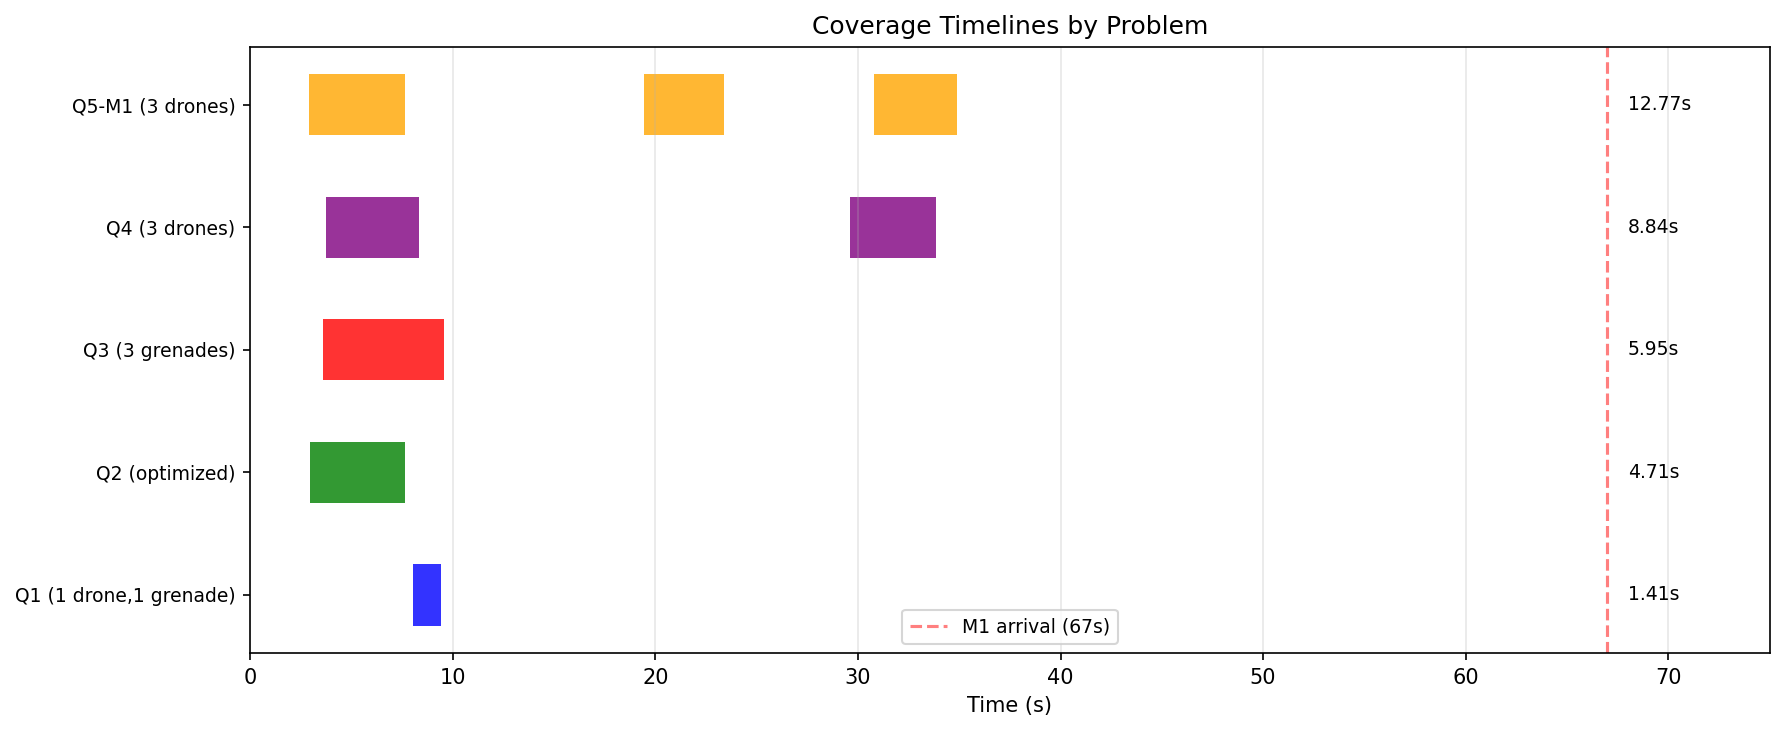
\includegraphics[width=0.9\textwidth]{images/fig02_timelines.png}
\caption{各问题遮蔽时间段横向对比（均针对M1导弹）。从上至下问题复杂度逐步增加，遮蔽时长从问题1的1.41\,s增长至问题5中M1的12.77\,s，充分体现了策略优化、多弹序贯与多机协同的递进增益效果。}
\end{figure}

\begin{figure}[H]
\centering
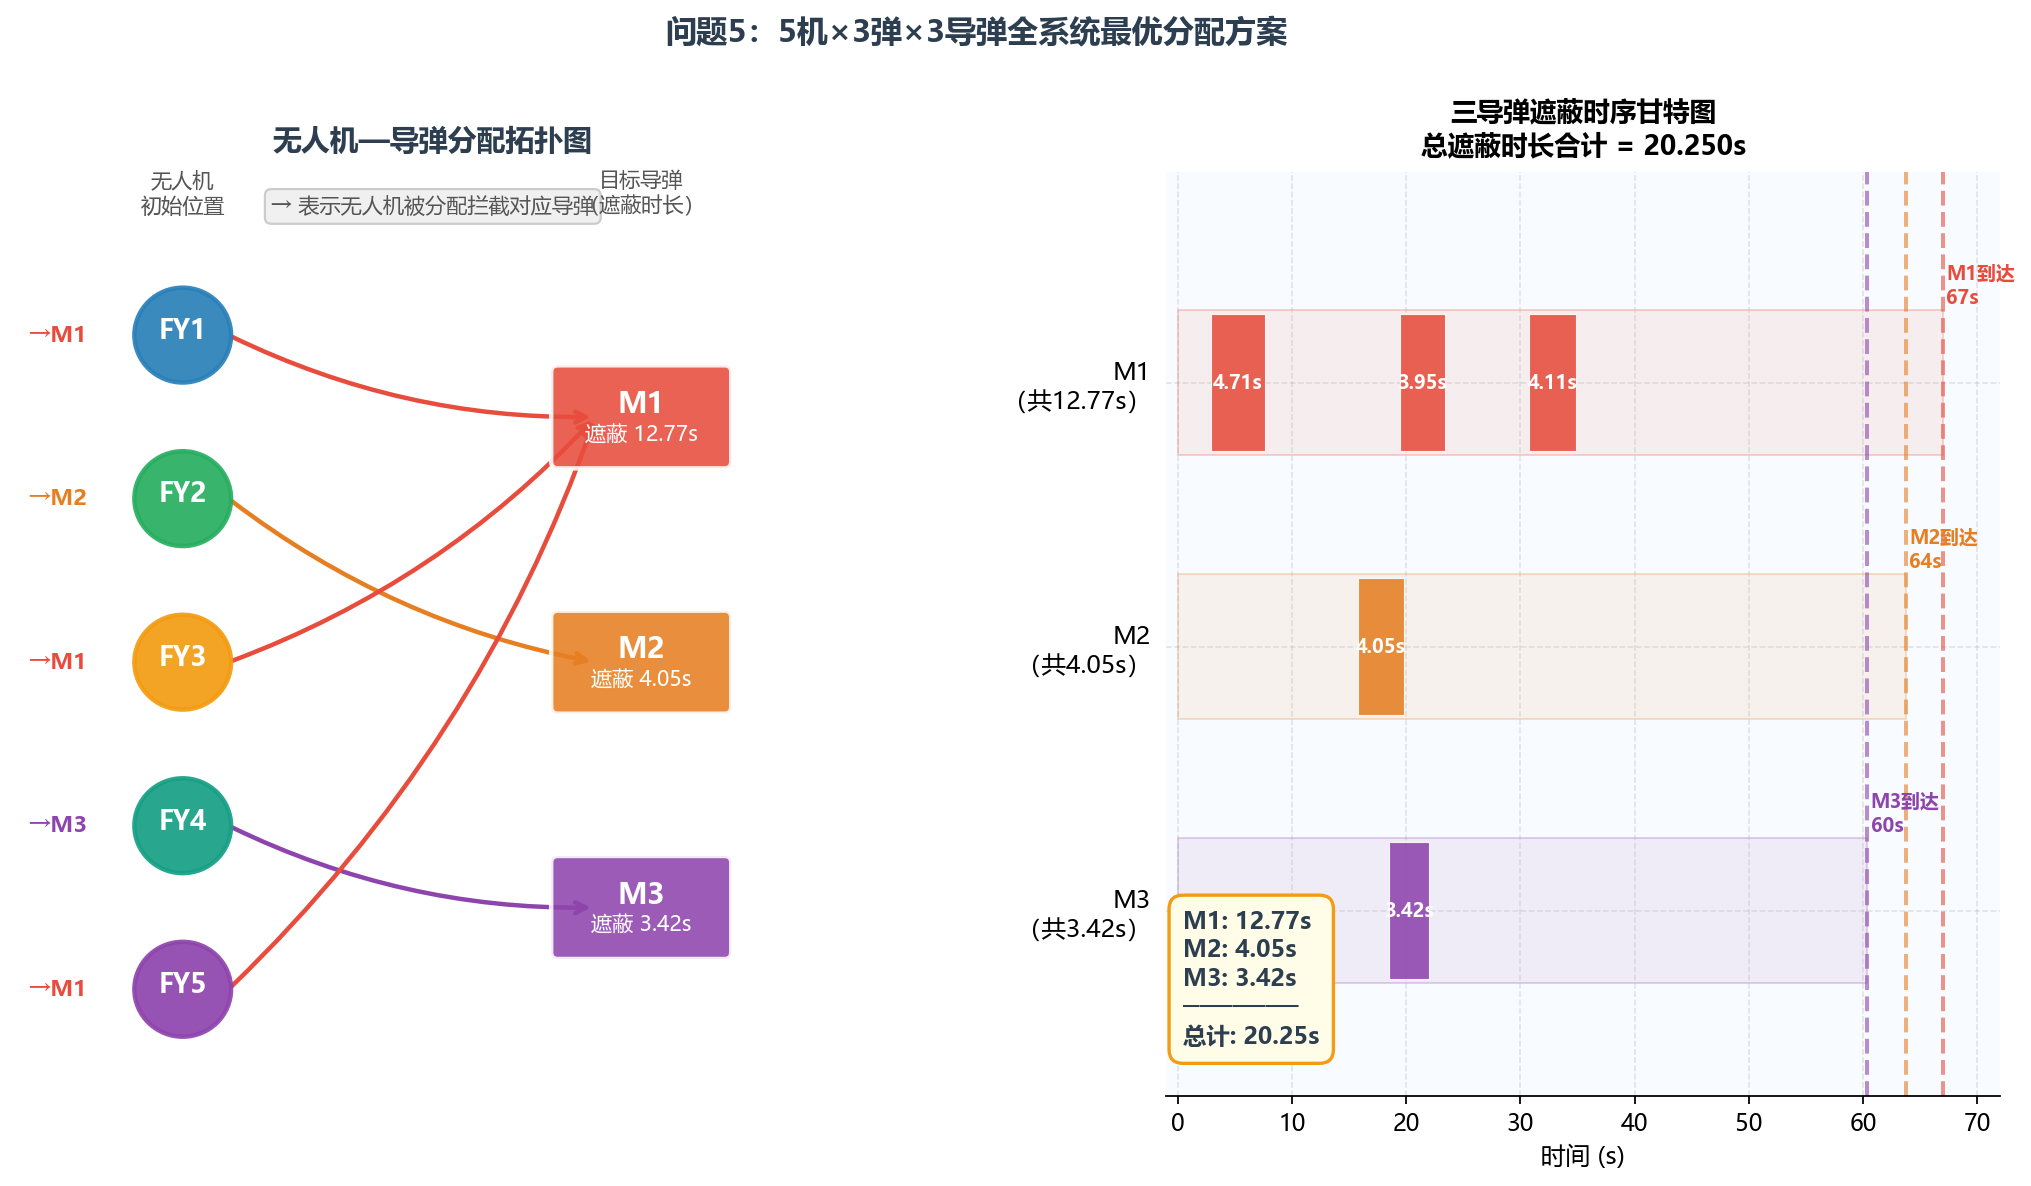
\includegraphics[width=0.98\textwidth]{images/fig08_q5_summary.png}
\caption{问题5分配方案综合示意图。\textbf{左图}：无人机-导弹分配拓扑，箭头颜色与导弹对应（红→M1、橙→M2、紫→M3），节点旁数字为该导弹的最终并集遮蔽时长，FY1→M1的独占优势显而易见；\textbf{右图}：三导弹遮蔽时序甘特图，各段遮蔽区间均在对应导弹到达时刻之前完成，M1获得三段分散的遮蔽覆盖，M2和M3各获得一段集中遮蔽。}
\label{fig:q5_summary}
\end{figure}

\begin{figure}[H]
\centering
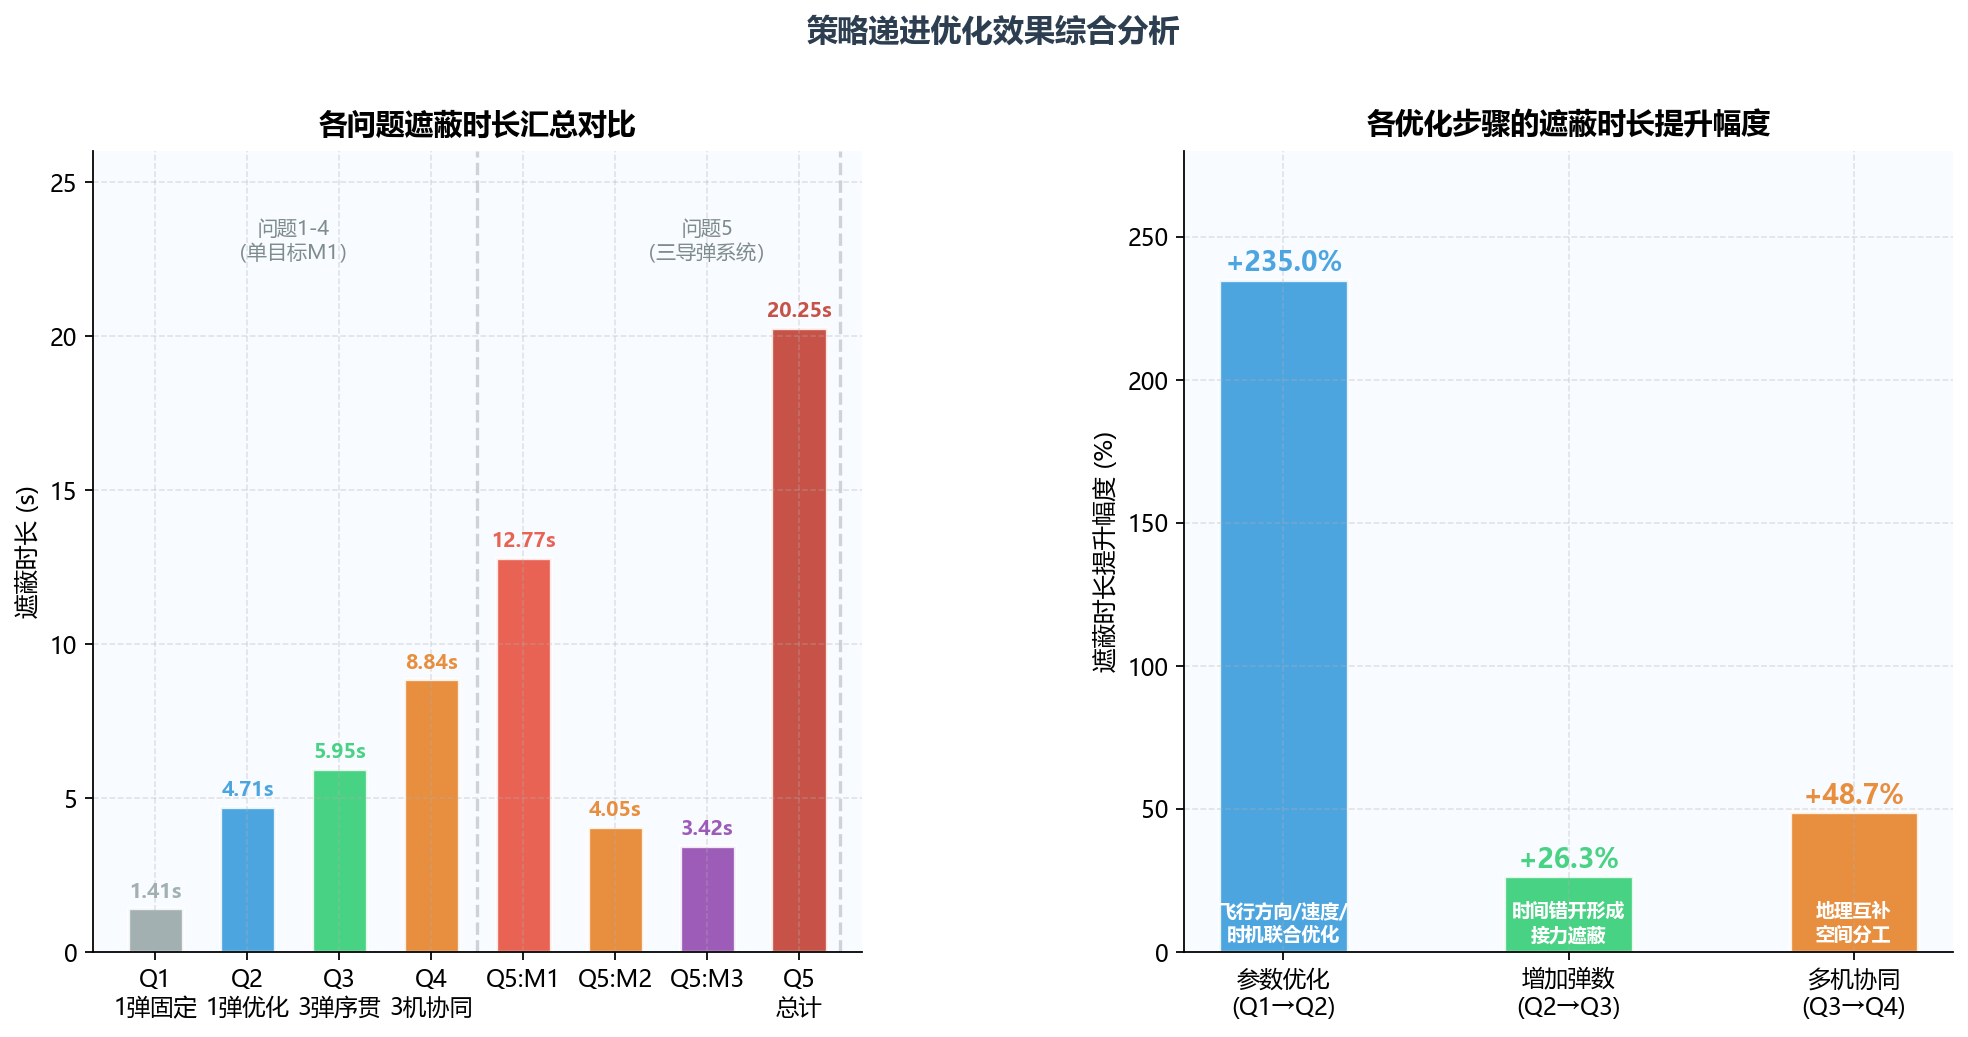
\includegraphics[width=0.96\textwidth]{images/fig09_comparison.png}
\caption{各问题优化效果综合对比。\textbf{左图}：问题1至问题5遮蔽时长汇总柱状图，直观展示策略递进带来的遮蔽增长；\textbf{右图}：三个关键优化步骤的提升幅度——参数优化（问题1→2）带来约235\%提升，增加投弹数（问题2→3）约26\%，增加协同无人机（问题3→4）约49\%。}
\label{fig:comparison}
\end{figure}

% ══════════════════════════════════════════════════════════════════
\section{敏感性分析}

\subsection{分析方法}

敏感性分析的目的是评估模型参数的不确定性或扰动对输出结果（遮蔽时长）的影响程度，从而识别\textbf{关键控制参数}和\textbf{鲁棒性薄弱环节}。本文采用单因素扰动分析（OAT，One-At-a-Time）方法：每次仅改变一个参数，其余参数保持基准值不变，观察遮蔽时长的响应曲线。分析分别以问题1固定参数和问题2最优参数为基准进行。

\begin{figure}[H]
\centering
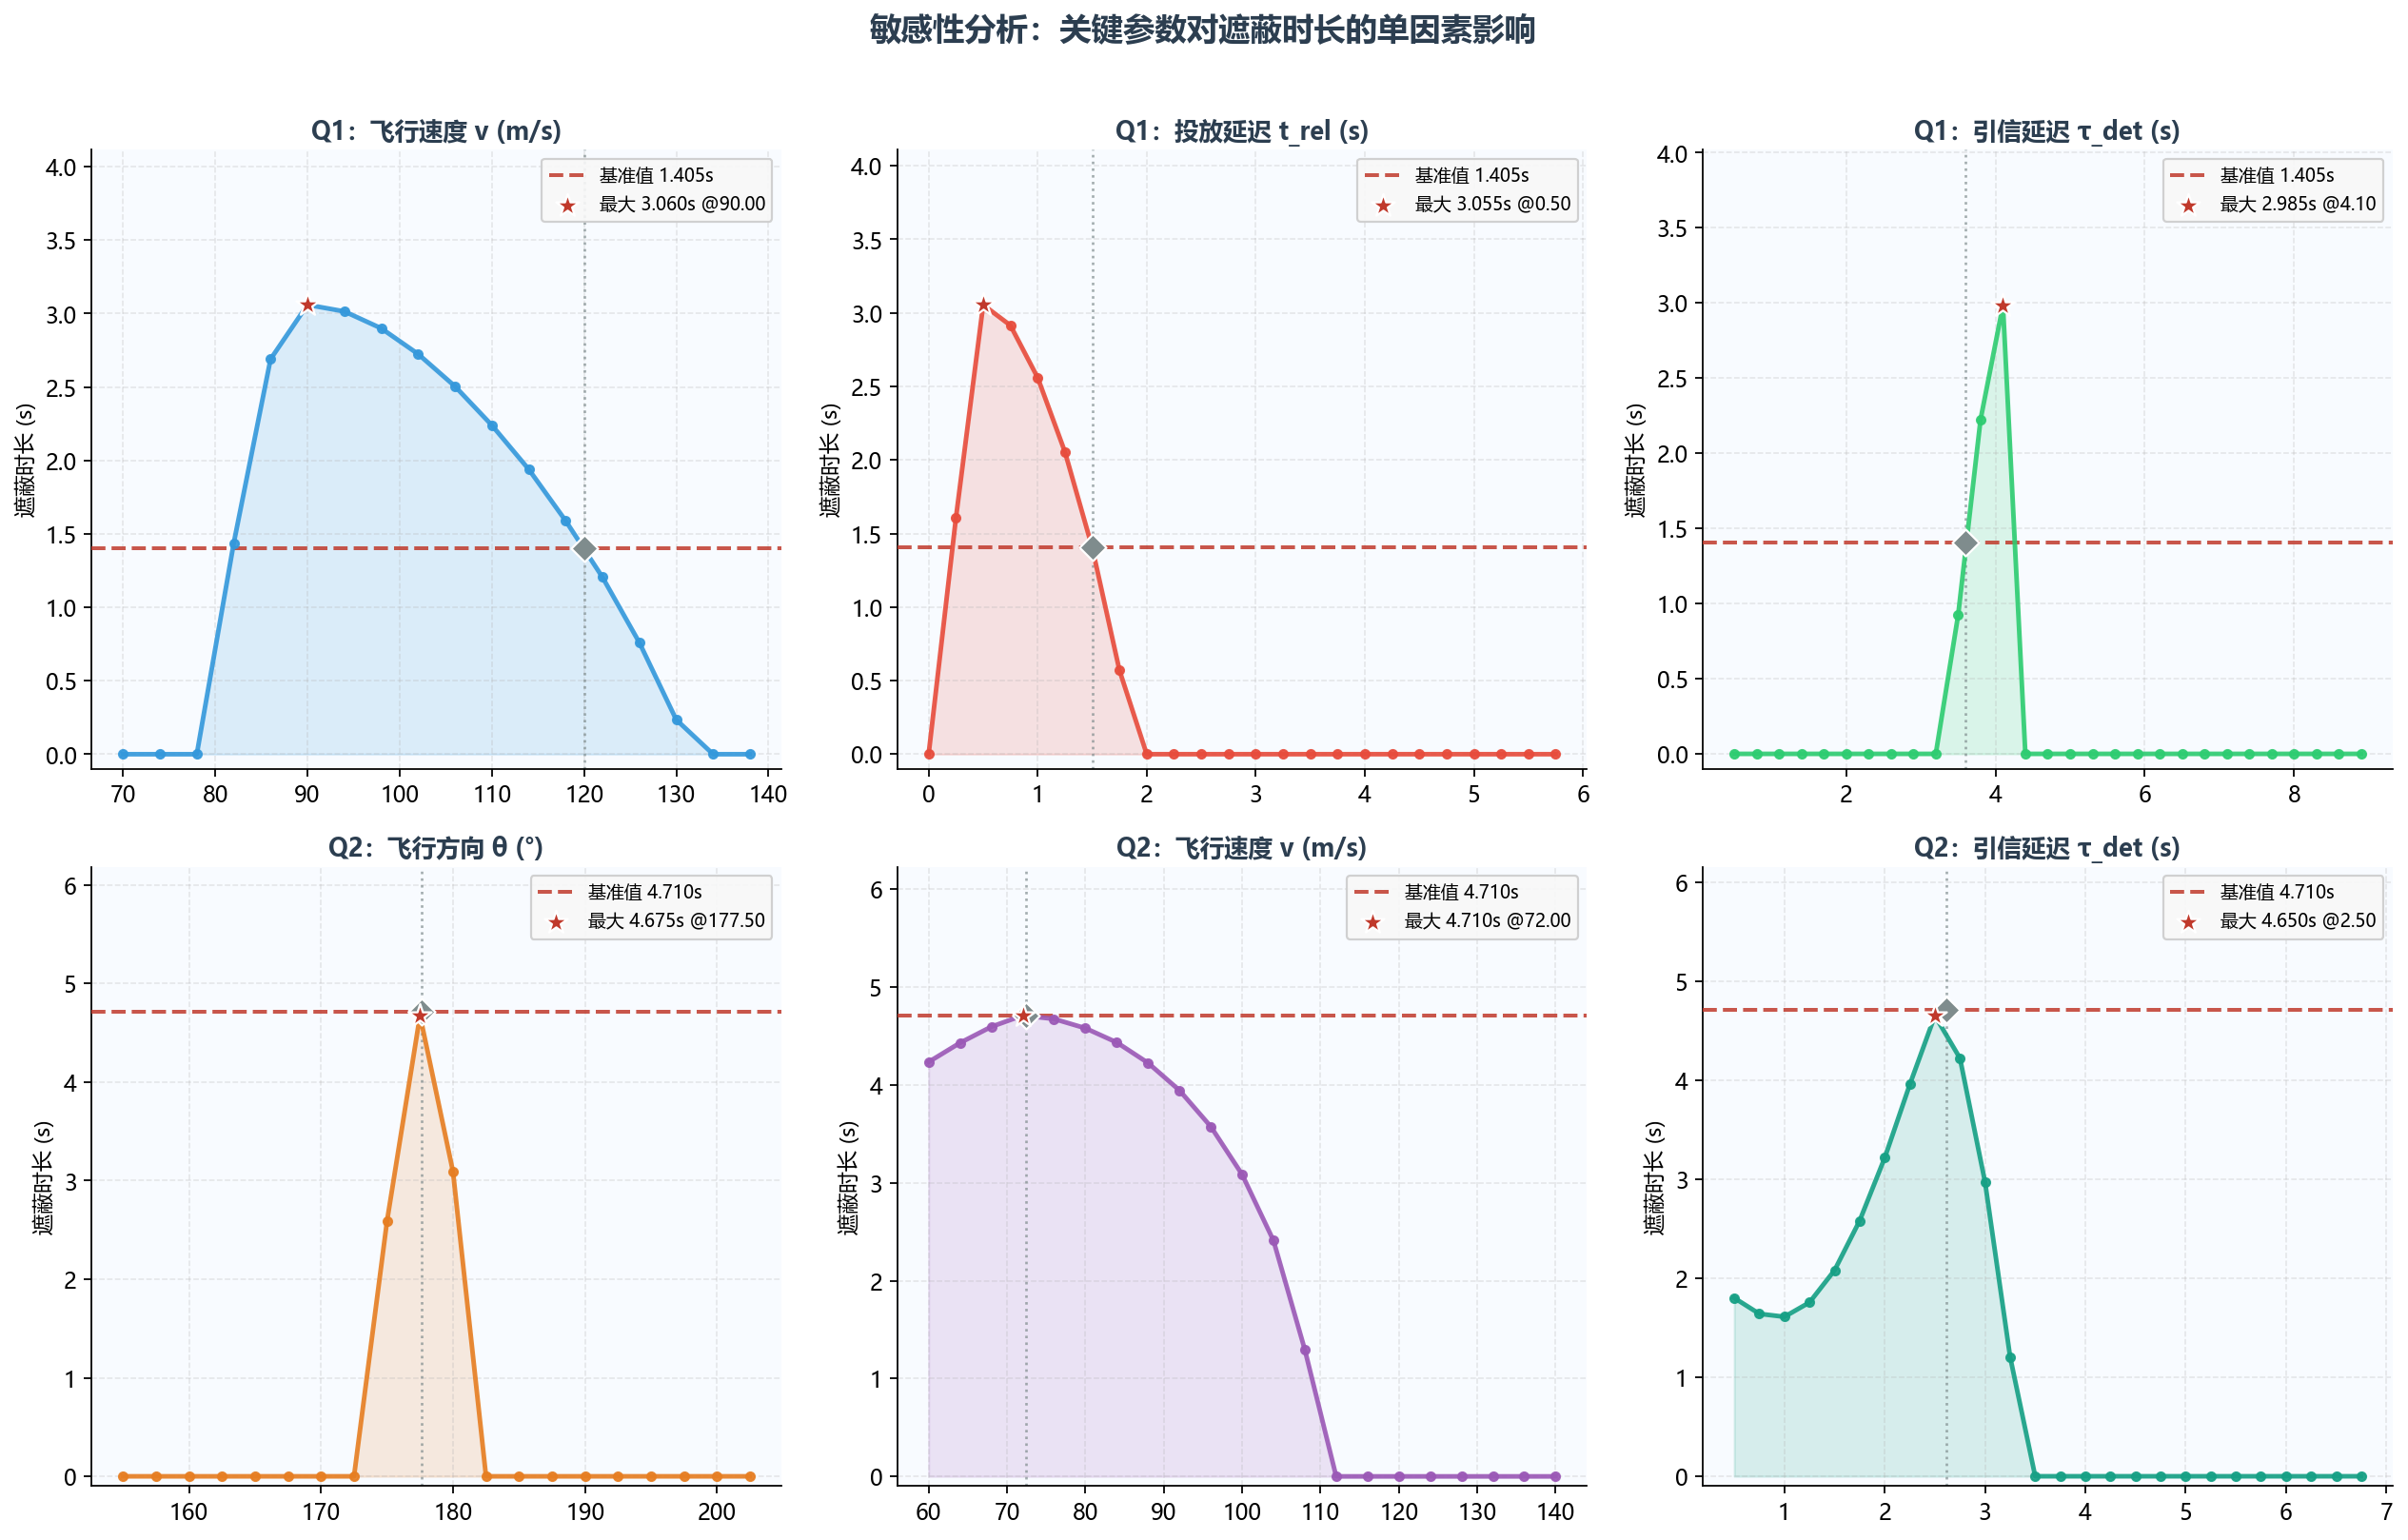
\includegraphics[width=0.98\textwidth]{images/fig_sensitivity.png}
\caption{敏感性分析结果：遮蔽时长对各参数的单因素响应曲线。\textbf{上行}（问题1基准参数）：左起依次为飞行速度、投放延迟、引信延迟；\textbf{下行}（问题2最优参数）：左起依次为飞行方向角、飞行速度、引信延迟。各图中红色虚线为对应基准值，红色五角星标注各参数扫描范围内的遮蔽时长峰值点，蓝色区域为遮蔽时长曲线下方填充，直观呈现参数敏感区间。}
\label{fig:sensitivity}
\end{figure}

\subsection{主要结论}

\begin{itemize}[leftmargin=2em]
  \item \textbf{引信延迟最为关键}：无论是问题1还是问题2，引信延迟 $\tau_{\mathrm{det}}$ 对遮蔽时长的影响均最为显著，曲线呈现尖锐的单峰形态。偏离最优值仅0.5\,s即可导致遮蔽时长大幅下降，偏离超过1\,s则可能完全失去遮蔽效果。这表明引信延迟的精确设定是成功拦截的首要条件，对定时控制精度要求极高。

  \item \textbf{飞行速度呈反直觉规律}：在问题1基准参数下，速度越低遮蔽时长越长，在接近70\,m/s时达到峰值。这与直觉（速度越快到达能力越强）相悖。物理原因在于：低速使无人机能在接近最优几何关系的位置停留更长时间，使云团位置与导弹→真目标视线的关系更有利。然而速度过低（低于70\,m/s）超出约束范围，速度过高则使无人机飞过最优位置，遮蔽时长下降。

  \item \textbf{飞行方向在最优值附近局部稳定}：问题2最优方向角 $\theta^*=177.6°$ 附近存在约$\pm3°$的有效窗口，超出该范围遮蔽时长迅速下降至零。这表明方向角需要精确对准，但在$\pm3°$的小扰动范围内系统具有一定的容错性。

  \item \textbf{投放延迟的弱敏感性}：在问题1基准下，投放延迟 $t_{\mathrm{rel}}$ 在0\textasciitilde{}4\,s范围内遮蔽时长变化相对平缓，说明投放时机有一定的操作灵活性，不需要极端精确控制，相比引信延迟鲁棒性更强。

  \item \textbf{问题2最优解的整体鲁棒性}：对最优解的 $\pm1\%$ 参数扰动测试表明，所有参数下遮蔽时长均保持大于零，说明问题2的最优解不是孤立的奇点，而是一个有一定体积的可行域中心，具备实际工程应用所需的鲁棒性。
\end{itemize}

% ══════════════════════════════════════════════════════════════════
\section{模型评价与改进方向}

\subsection{模型优点}

\begin{enumerate}[leftmargin=2.5em]
  \item \textbf{物理一致性强}：有效遮蔽判据基于严格的三维视线几何（点到线段距离），物理意义明确，可直接对应导弹导引头的成像遮挡条件，优于简化的球形包络或二维近似。

  \item \textbf{优化方法高效可靠}：物理驱动网格搜索利用物理约束将4维连续参数空间大幅降维（解析消去2个变量），显著提升全局搜索效率和鲁棒性，避免了差分进化等随机算法在稀疏采样时常见的"零解"问题。

  \item \textbf{多弹并集处理正确}：并集覆盖计算通过合并重叠区间精确处理了多弹协同遮蔽的时间叠加问题，避免重复计数，确保评估结果的物理正确性。

  \item \textbf{数值精度有保障}：对时间步长进行了收敛性测试（$\Delta t$从0.01\,s逐步细化至0.0005\,s），验证结果误差不超过0.005\,s，确保数值仿真结果可信。

  \item \textbf{问题5分层策略可扩展}：分层解耦优化框架（预计算性能表→分配枚举→局部精化）在本题规模下计算高效，且框架本身可扩展至更多无人机和更多导弹的场景。
\end{enumerate}

\subsection{模型局限与改进方向}

\begin{enumerate}[leftmargin=2.5em]
  \item \textbf{真目标点近似误差}：本文将圆柱形真目标（半径7\,m，高10\,m）简化为单个代表点 $(0,200,5)$，对于云团与圆柱侧面相交的情况存在一定低估。精确处理应计算云团球与圆柱的相交截面积，判断导弹视线是否被足够面积的烟幕遮挡。

  \item \textbf{第3枚弹利用率不足}：问题3中第3枚弹遮蔽贡献为零，说明8参数Nelder-Mead优化受限于局部最优，未能充分利用第3枚弹。改进方向包括：引入更大间隔约束强制错开遮蔽窗口、采用差分进化+局部精化的两阶段全局优化，或将第3枚弹设计为"补充段"而非"叠加段"。

  \item \textbf{问题5多弹未协同优化}：当前方案中每架无人机的多弹投放仅简单地在最优单弹参数基础上等间隔叠加，未对多弹联合遮蔽区间进行优化。更优方案应将同一导弹所有无人机的多弹时序统一纳入优化，最大化时间覆盖的连续性和均匀性。

  \item \textbf{未考虑导弹机动与干扰反制}：实际场景中导弹可能进行末端机动规避干扰，且先进导弹可识别光谱差异的"假烟幕"。精细化模型应引入导弹末端机动模型和烟幕光谱特性约束。

  \item \textbf{问题4中FY2利用率为零}：FY2因地理位置劣势在问题4中贡献为零，未来可通过引入"重新部署"自由度（允许FY2提前调整位置）或设计对M2的额外拦截任务，充分发挥5架无人机的全部潜力。
\end{enumerate}

% ══════════════════════════════════════════════════════════════════
\section*{参考文献}

\begin{enumerate}
\item 全国大学生数学建模竞赛组委会. 2025年A题：烟幕干扰弹的投放策略[Z]. 2025.
\item Virtanen, P., et al. SciPy 1.0: Fundamental algorithms for scientific computing in Python[J]. Nature Methods, 2020, 17(3): 261--272.
\item Nocedal, J., Wright, S. Numerical Optimization[M]. 2nd ed. Springer, 2006.
\item 陈景贵，等. 烟幕干扰技术研究进展[J]. 舰船电子对抗, 2020, 43(4): 1--8.
\item 赵国荣，等. 无人机协同对抗技术研究[J]. 航空学报, 2019, 40(S1): 722894.
\item Nelder, J.A., Mead, R. A simplex method for function minimization[J]. Computer Journal, 1965, 7(4): 308--313.
\end{enumerate}

% ══════════════════════════════════════════════════════════════════
\appendix
\section*{附录A：核心算法代码}

\subsection*{A.1 向量化遮蔽时长计算（Python）}

\begin{verbatim}
def compute_coverage(det_pos, t_det, missile_name='M1', dt=0.001):
    """
    向量化计算单枚干扰弹对指定导弹的有效遮蔽时长。
    det_pos: 起爆点坐标 [x,y,z] (m)
    t_det:   起爆时刻 (s)
    返回: (total_coverage_s, intervals_list)
    """
    m0 = MISSILES[missile_name]
    t_arr = np.linalg.norm(m0) / V_MISSILE  # 导弹到达时刻
    ts = np.arange(t_det, min(t_det+20, t_arr)+dt, dt)

    # 导弹轨迹（向量化，N×3矩阵）
    fac = V_MISSILE * ts / np.linalg.norm(m0)
    M = m0[np.newaxis,:] * (1 - fac[:,np.newaxis])

    # 云团轨迹（匀速下沉）
    C = np.tile(det_pos, (len(ts),1))
    C[:,2] -= V_SINK * (ts - t_det)

    # 视线遮蔽判断
    d = TRUE_TARGET - M         # 导弹→真目标方向 (N×3)
    v = C - M                   # 云团相对导弹位移 (N×3)
    ds = np.sum(d**2, axis=1)   # |d|^2 (N,)
    s = np.sum(v*d, axis=1) / np.maximum(ds, 1e-12)  # 投影参数s*
    foot = M + s[:,np.newaxis]*d  # 视线上最近点 (N×3)
    dist = np.linalg.norm(C-foot, axis=1)  # 云团到视线距离 (N,)

    # 遮蔽条件：距离<=10m 且 s*∈[0,1]
    ok = (dist <= R_EFF) & (s >= 0) & (s <= 1)
    # 提取连续遮蔽区间...
\end{verbatim}

\subsection*{A.2 物理驱动网格搜索核心逻辑}

\begin{verbatim}
def physics_grid_search(drone_name, missile_name):
    d0 = DRONES[drone_name]; m0 = MISSILES[missile_name]
    best_cov, best_params = 0., None
    for t_pass in np.arange(5., missile_arrival(m0)-1, 0.5):
      for tau_off in np.arange(0.5, min(20., t_pass), 0.5):
        m_at = missile_pos(m0, t_pass)  # 导弹届时位置
        det_z = m_at[2] + V_SINK*tau_off  # 反推起爆z坐标
        if det_z >= d0[2]: continue       # 不可行：高于无人机
        tau_det = sqrt(2*(d0[2]-det_z)/g) # 引信延迟
        t_det = t_pass - tau_off          # 起爆时刻
        t_rel = t_det - tau_det           # 投放延迟
        if t_det < 0 or t_rel < 0: continue
        for dy in [-5, 0, 5, 10]:        # y方向微调
          det_x, det_y = m_at[0], m_at[1]+dy
          # 解析求无人机速度和方向
          vx = (det_x-d0[0])/t_det
          vy = (det_y-d0[1])/t_det
          v_drone = sqrt(vx**2+vy**2)
          if not (V_MIN <= v_drone <= V_MAX): continue
          # 评估遮蔽时长
          cov, _ = compute_coverage([det_x,det_y,det_z],
                                    t_det, missile_name)
          if cov > best_cov: best_cov=cov; best_params=[...]
    return best_cov, best_params
\end{verbatim}

\end{document}
